\svnidlong
{$HeadURL$}
{$LastChangedDate$}
{$LastChangedRevision$}
{$LastChangedBy$}
\svnid{$Id$}


% preamble

In this chapter we review recommendations for final states of \MET{} recoiling against a particle extracted from initial state radiation. While the recommendations are general, the discussions in this chapter are made based on the monojet final state. These studies and studies in subsequent sections are based on simulation of the models with the generators implementation recommended in each section and provided in a companion CERN SVN repository. Further details on the mono-$\gamma/W/Z$ final states from boson radiation are discussed in Sec.~\ref{sec:bosonrad}.


\section{Vector and axial vector mediator, \schannel exchange}
\label{sec:monojet_V}


A simple extension of the Standard Model (SM) is an
additional $U(1)$ gauge symmetry, where a dark matter (DM)
candidate particle has charges only under this new group.
Assuming that some SM particles are also charged under
this group, then a new gauge boson can mediate interactions
between the SM and DM.   


%Lagrangian
We consider the case of a DM particle that is a Dirac fermion and where the production proceeds via the exchange of a spin-1 mediator in
the \schannel, illustrated in Fig.~\ref{fig:OP}.

\begin{figure}[h!]
\centering
  \unitlength=0.005\textwidth
  \vspace{0.5\baselineskip}
  \begin{feynmandiagram}[modelVmonojetParameters]
    \fmfleft{i1,i2}
    \fmfright{o1,o2}
    \fmftop{isr}
    \fmfbottom{pisr}
    % \fmf{dashes,tension=0.6,label={$\substack{{\Large V,,A}\\(m_{med},,\Gamma_{min,,med})}$}}{v1,v2}
    \fmf{wiggly,tension=0.6,label={\Large $V,,A(\mMed)$}}{v1,v2}
    \fmf{fermion}{o2,v2,o1}
    \fmf{fermion}{i2,visr,v1}
    \fmf{plain}{v1,pvisr,i1}
    \fmf{fermion,tension=0}{v1,i1}
    \fmfdot{v1,v2}
    \fmflabel{\Large ${g_q}$}{v1}
    \fmflabel{\Large ${g_{DM}}$}{v2}
    \fmflabel{\Large ${\bar{q}}$}{i1}
    \fmflabel{\Large ${q}$}{i2}
    \fmflabel{\Large ${\bar{\chiDM}(\mDM)}$}{o1}
    \fmflabel{\Large ${\chiDM(\mDM)}$}{o2}
    \fmf{gluon,tension=0}{visr,isr}
    \fmf{phantom,tension=0}{pvisr,pisr}
    \fmflabel{\Large ${g}$}{isr}
  \end{feynmandiagram}
%\caption[][\baselineskip]{Representative Feynman
\caption{Representative Feynman
diagram showing the pair production of dark matter particles in association with a parton from the initial state via a vector or axial-vector mediator.
The cross section and kinematics depend upon
the mediator and dark matter masses, and the mediator couplings to dark matter and quarks respectively: ($\mMed ,\, \mDM ,\, \gDM ,\, \gq)$. }
\label{fig:OP}
\setfloatalignment{t}
  \vspace{0.5\baselineskip}
\end{figure}

We consider two models with vector and axial-vector couplings
between the spin-1 mediator and SM and DM fields, with
the corresponding interaction Lagrangians:
\begin{align}
\label{eq:AV} 
\mathcal{L}_{\mathrm{vector}} &= \gq \sum_{q={u,d,s,c,b,t}}  \Zprime_{\mu} \bar{q}\gamma^{\mu}q + \gDM \Zprime_{\mu} \bar{\chiDM}\gamma^{\mu}\chiDM \\
\mathcal{L}_{\rm{axial-vector}} &= \gq \sum_{q={u,d,s,c,b,t}}  \Zprime_{\mu} \bar{q}\gamma^{\mu}\gamma^5q + \gDM \Zprime_{\mu} \bar{\chiDM}\gamma^{\mu}\gamma^5\chiDM.
\end{align}
The coupling \gq is assumed to be universal to all quarks. 
It is also possible to consider other models in which mixed vector and axial-vector couplings are considered, 
for instance the couplings to the quarks are axial-vector whereas those to DM are vector. We recommend the models with
pure vector couplings or pure axial-vector couplings.
\Todo{Studies have been performed to see if the case of a mixed coupling can be simply extracted from the other models by some reweighting procedure to take account of the difference in cross section. This would assume that the difference between the pure and mixed couplings case does not affect the kinematics of the event. Note, though, that in the mediator rest frame, the angular distribution of the DM relative to the mediator direction of motion has the form: $1+z^2+2*C*z$ ($z=\cos\theta$), with the second term only present in the mixed case. This may lead to acceptance differences.}
%Definition of minimal width
As mentioned in the introduction, when no additional visible or invisible decays contribute to the width of the mediator, 
the minimal width is fixed by the choices of couplings $\gq$ and $\gDM$. The effect of larger 
widths is discussed on page \pageref{paragraph:nonminimalwidth}. 
For the vector and axial-vector models, the minimal width is

\begin{equation}
%\Gamma_{\rm{min}}=\Gamma_{\bar{\chiDM}\chiDM} + \sum_{q}N_{c}\Gamma_{\bar{q}q}
\Gamma_{\rm{min}}^{V/A}=\Gamma_{\bar{\chiDM}\chiDM}^{V/A} + \sum_{q}\Gamma_{\bar{q}q}^{V/A}.
\label{eq:monojet_min}
\end{equation}

The leading order expressions for the partial widths are:

\begin{align}
\Gamma_{\bar{\chiDM}\chiDM}^{\rm{V}}&=\frac{\gDM^2 \mMed}{12\pi}\left(1+\frac{2 \mDM^2}{\mMed^2} \right)\beta_{DM} \theta(\mMed-2\mDM)\\
\Gamma_{\bar{q}q}^{\rm{V}}&= \frac{3 \gq^2 \mMed}{12\pi}\left(1+\frac{2 m_q^2}{\mMed^2} \right)\beta_q \theta(\mMed-2m_q)\\
\Gamma_{\bar{\chiDM}\chiDM}^{\rm{A}}&=\frac{\gDM^2 \mMed}{12\pi} \beta_{DM}^{3/2} \theta(\mMed-2\mDM)\\
\Gamma_{\bar{q}q}^{\rm{A}}&= \frac{3 \gq^2 \mMed}{12\pi}\beta_q^{3/2} \theta(\mMed-2m_q)\;,
\label{eq:GammaV}
\end{align}
$\theta(x)$ denotes the Heaviside step function, and
$\beta_f=\sqrt{1-\frac{4 m_f^2}{\mMed^2}}$ is the velocity of the
fermion $f$ in the mediator rest frame.
Note the color factor 3 in the quark terms.
Figure\,\ref{fig:monojet_width_V} shows the minimal width as a function of mediator mass for both vector and axial-vector mediators assuming
\gq=\gDM=1. With this choice of the couplings, the dominant contribution to the minimal width comes from the quarks due to the color factor enhancement and
the large number of them.

\begin{figure}
\centering
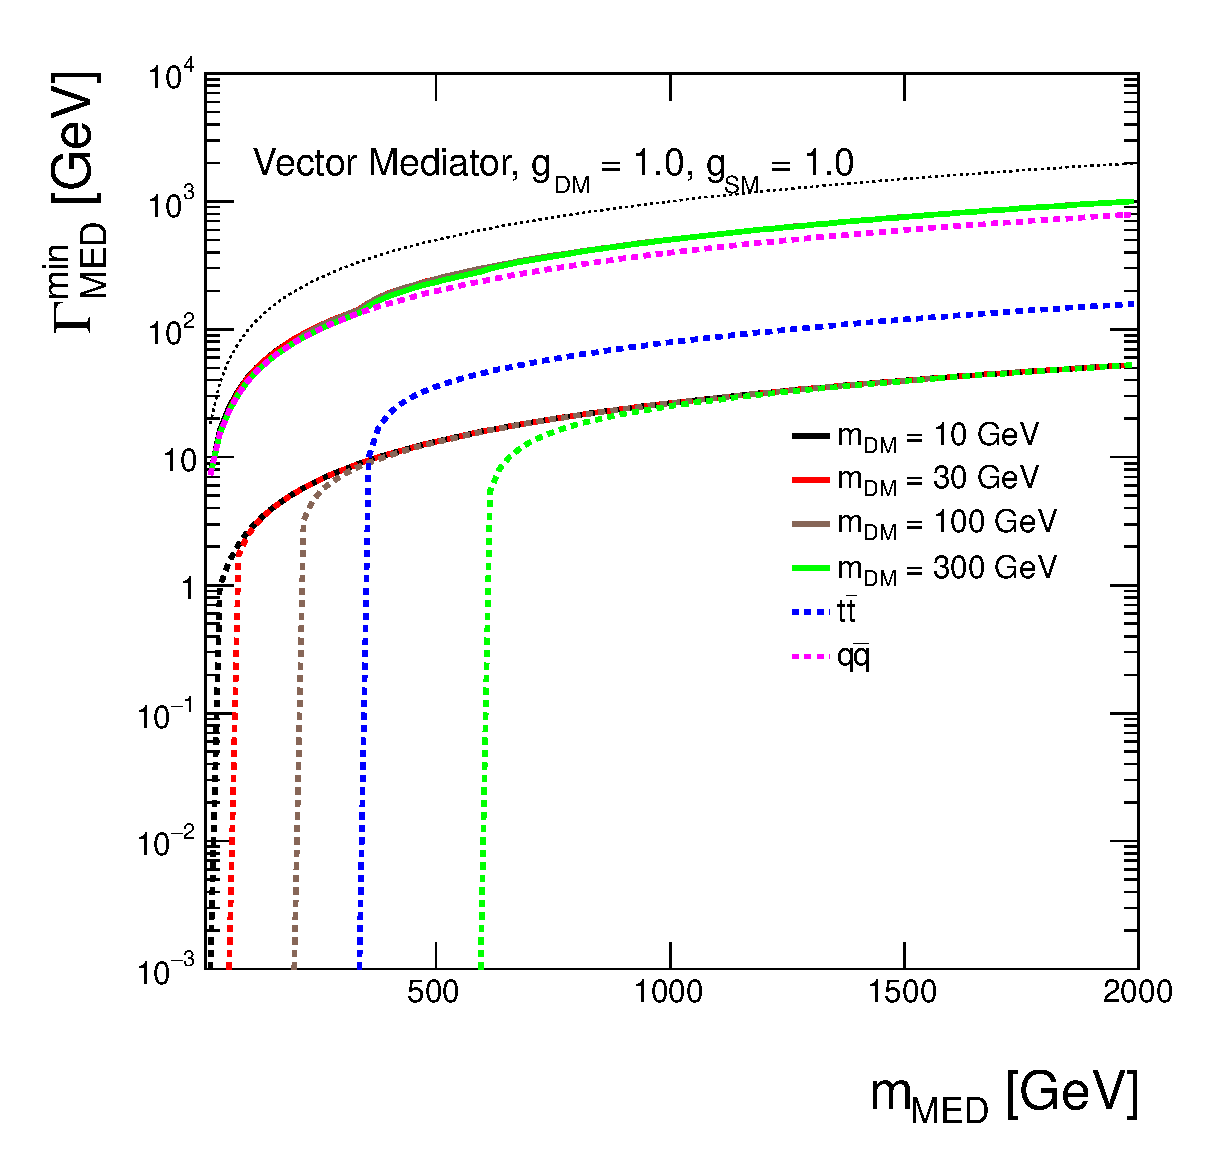
\includegraphics[width=0.45\textwidth]{figures/monojet/width_V.eps}
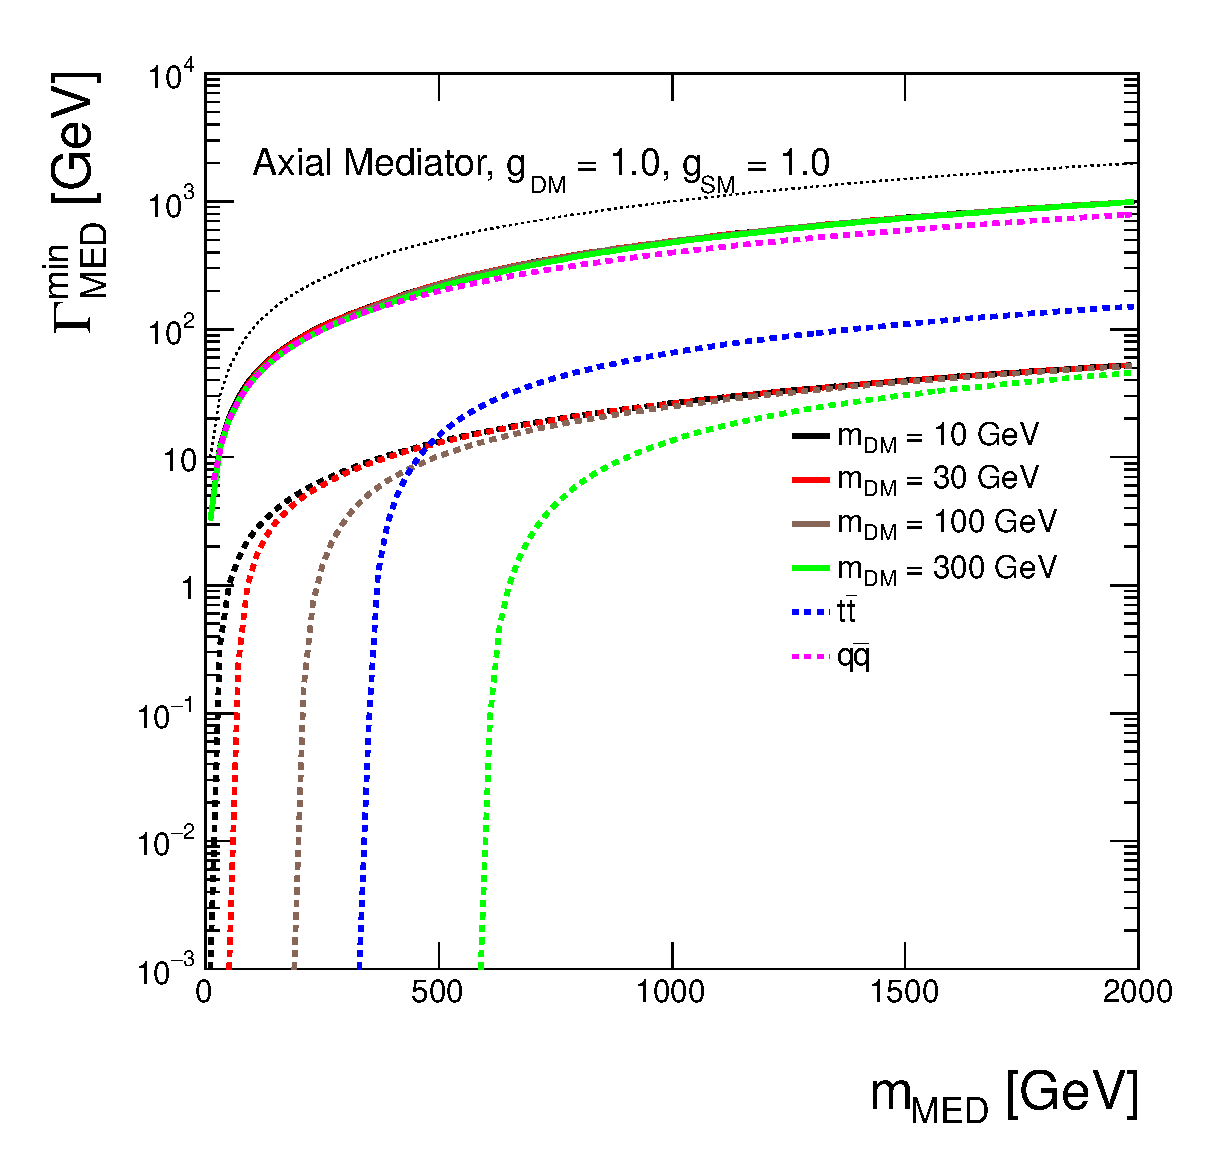
\includegraphics[width=0.45\textwidth]{figures/monojet/width_A.eps}
\caption{Minimal width as a function of mediator mass for vector and axial-vector mediator assuming couplings of 1. The total width is shown as solid lines for Dark Matter masses of 10~\gev, 30~\gev, 100~\gev and 300~\gev in black, red, brown and green, respectively. The individual contributions from Dark Matter are indicated by dotted lines with the same colors. The contribution from all quarks but top is shown as magenta dotted line and the contribution from top quarks only is illustrated by the dotted blue line. The dotted black line shows the extreme case $\Gamma_{\rm{min}}=\mMed$.}
\label{fig:monojet_width_V}
\end{figure}

The two simplified models described here have four free parameters: mediator mass $\mMed$, Dark Matter mass $\mDM$, coupling of the mediator to quarks $\gq$ and coupling of the mediator to Dark Matter $\gDM$. See~\cite{Buchmueller:2014yoa} for a thorough discussion. In order to determine an optimal choice of the parameter grid for presentation of the early Run-2 results, dependencies of the kinematic quantities and cross sections on the individual parameters have been studied. The following paragraphs list the main observations from the scans over the parameters that support the final proposal for the parameter grid.


\paragraph{Scan over the couplings}

Figure\,\ref{fig:monojet_scan_V_g} In order to study the dependence on the coupling strength, samples were generated where a pair of \mDM=10~\gev Dark Matter particles are produced on-shell from the mediator of \mMed=1~\tev.
No differences in the shape of the \MET distribution are observed for the different choices of the coupling strength.
This is a generator-level prediction with no kinematic selections or detector simulation. Coupling values in the scan range 0.1--1.45, holding $\gq=\gDM$, correspond to a rough estimate of the lower sensitivity of mono-jet analyses and a maximum coupling value such that $\Gamma_{\rm{min}} < \mMed$.
Based on similar findings for different choices of
\mMed and \mDM, we conclude that the shapes of
kinematic distributions are not altered
by coupling variations, either for the on-shell Dark Matter production where $\mMed>2\mDM$,
or for the off-shell Dark Matter production where $\mMed<2\mDM$. Only the production cross sections change.
Differences in kinematic distributions are expected only close to the transition region where both on-shell and off-shell decays occur.
%TODO clarify slide 9 and 10 in https://indico.cern.ch/event/389275/contribution/1/material/slides/0.pdf
%TODO check explicitly for V and A (generate corresponding samples)
\begin{figure}
\centering
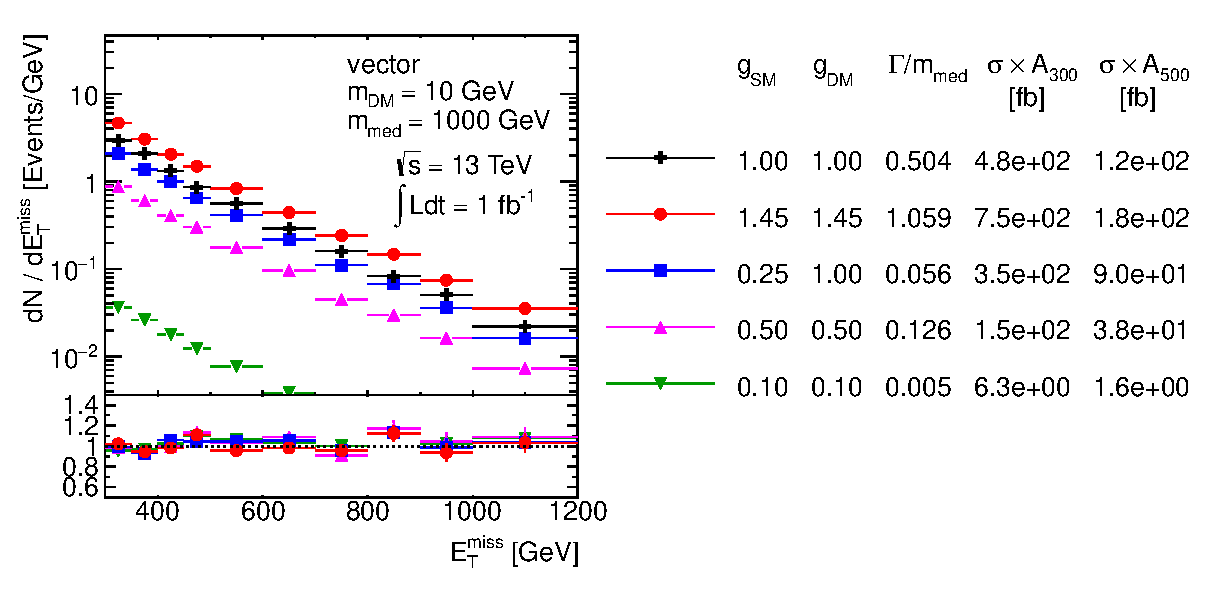
\includegraphics[width=0.9\textwidth]{figures/monojet/scan_g_V_10_1000.eps}
\caption{Scan over couplings. The $\MET$ distribution is compared for the vector mediator models using the parameters as indicated. Ratios of the normalized distributions with respect to the first one are shown. $A_{300}$ and $A_{500}$ in the table denote the acceptance of the $\MET>300$~\gev and $\MET>500$~\gev cut, respectively.}
\label{fig:monojet_scan_V_g}
\end{figure}

One situation requiring a careful consideration
is the case of 
extremely heavy and narrow mediators, which can arise for
small coupling strengths.
Upon close examination, it was determined that this case is
not peculiar.  However, the complete story is a cautionary tale
about understanding the details of the generator tools.
Figure\,\ref{fig:monojet_narrow} suggests a change in the shape of the
$\MET$ distribution for a \mMed=5~\tev mediator
once $\Gamma_{\rm{min}}/\mMed$ is of the order of a percent or lower.
This, however, does not come from physics, but is a consequence of under-sampling phase space in the generator implementation,
where a cutoff for the regions far away from the mediator mass is generally used. One must take care to correctly set the width of the Breit-Wigner used for the sampling.
This is illustrated in Fig.\,\ref{fig:monojet_mchichi} showing the invariant mass of the Dark Matter pair in the samples generated for a \mMed=7~\tev mediator
with different coupling strengths.
In all cases, it is expected to observe a peak around the mediator mass with a tail extending to $m_{\bar{\chiDM}\chiDM}\rightarrow0$, significantly enhanced by parton distribution functions at low Bjorken $x$. For coupling strength 1 and 3, the massive enhancement at $m_{\bar{\chiDM}\chiDM}\rightarrow0$ implies that
resonant production at $m_{\bar{\chiDM}\chiDM}=7$~\tev is statistically suppressed such that barely any events are generated there. However, for narrower mediators with couplings below 1, the peak around 7~\tev is clearly visible in the generated sample and the dominant tail at $m_{\bar{\chiDM}\chiDM}\rightarrow0$ is artificially cut off, leading to unphysical cross section predictions and kinematic shapes. This explains why the sample with the narrowest mediator in Fig.\,\ref{fig:monojet_narrow} is heavily suppressed in terms of production cross section and also gives different $\MET$ shape.
In general, for such extreme parameter choices
%as $\mMed=7$~\tev and $\Gamma_{\rm{min}}=36$~\gev,
the EFT model should give the correct answer. \Todo{Refer to results of ongoing study in Section 6.}
% In case the simplified model calculation does not reproduce the EFT result, the phase space generation of the simplified model has to be carefully examined in order to understand the cause of the problem. Fortunately, this is a rather academic discussion as such extreme corners of the parameter space are not going to be considered for presentation of Run-2 results.

%Uli: as fabio says, increasing bwcutoff might improve things in the case you are considering
%
%for a mediator with mass M = 7~\tev and width Gamma = 36~\gev, i think the correct way to do this calculation is to work in an EFT; this should give you the correct result
%
%in fact, if your simplified model calculation does not reproduce the EFT result for such extreme parameter choices, you have to carefully look at the phase-space generation of the simplified model calculation (as you did). at the end you probably have to tailor the phase-space generator of \madgraph, \powheg, etc. to get it right; this will be non-trivial since phase-space generation is an art! furthermore, one has to do this process 
%by process and the difficulties will increase from mono-jet to ttbar + \MET, etc. 

\begin{figure}
\centering
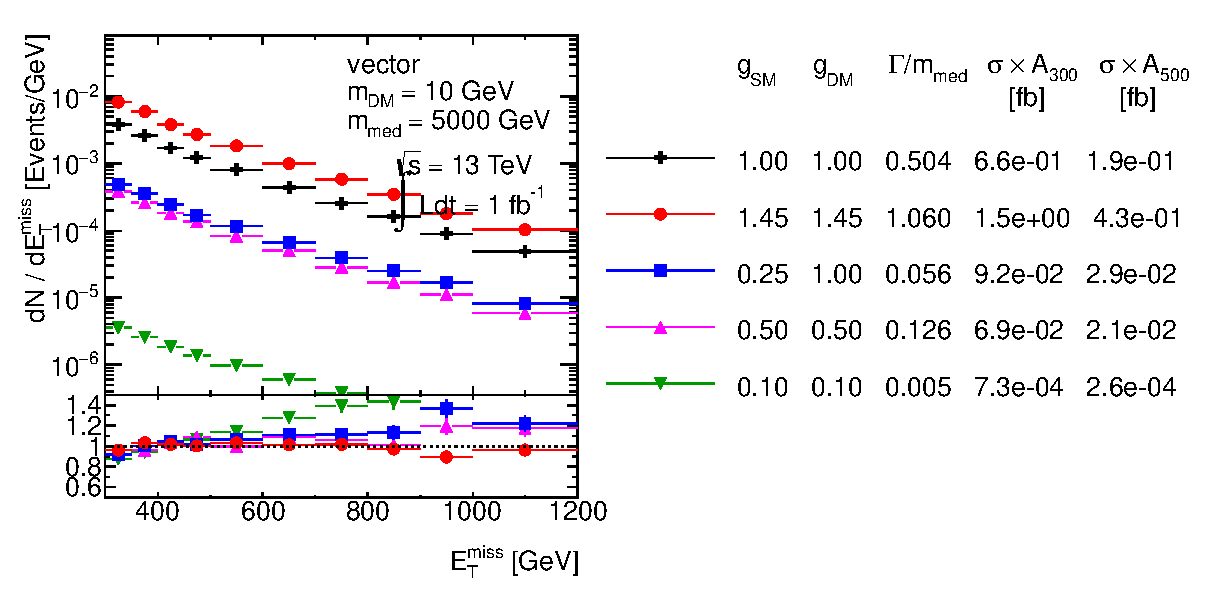
\includegraphics[width=0.9\textwidth]{figures/monojet/scan_g_V_10_5000.eps}
\caption{Scan over couplings. The $\MET$ distribution is compared for the vector mediator models using the parameters as indicated. Ratios of the normalized distributions with respect to the first one are shown. $A_{300}$ and $A_{500}$ in the table denote the acceptance of the $\MET>300$~\gev and $\MET>500$~\gev cut, respectively.}
\label{fig:monojet_narrow}
\end{figure}

\begin{figure}
\centering
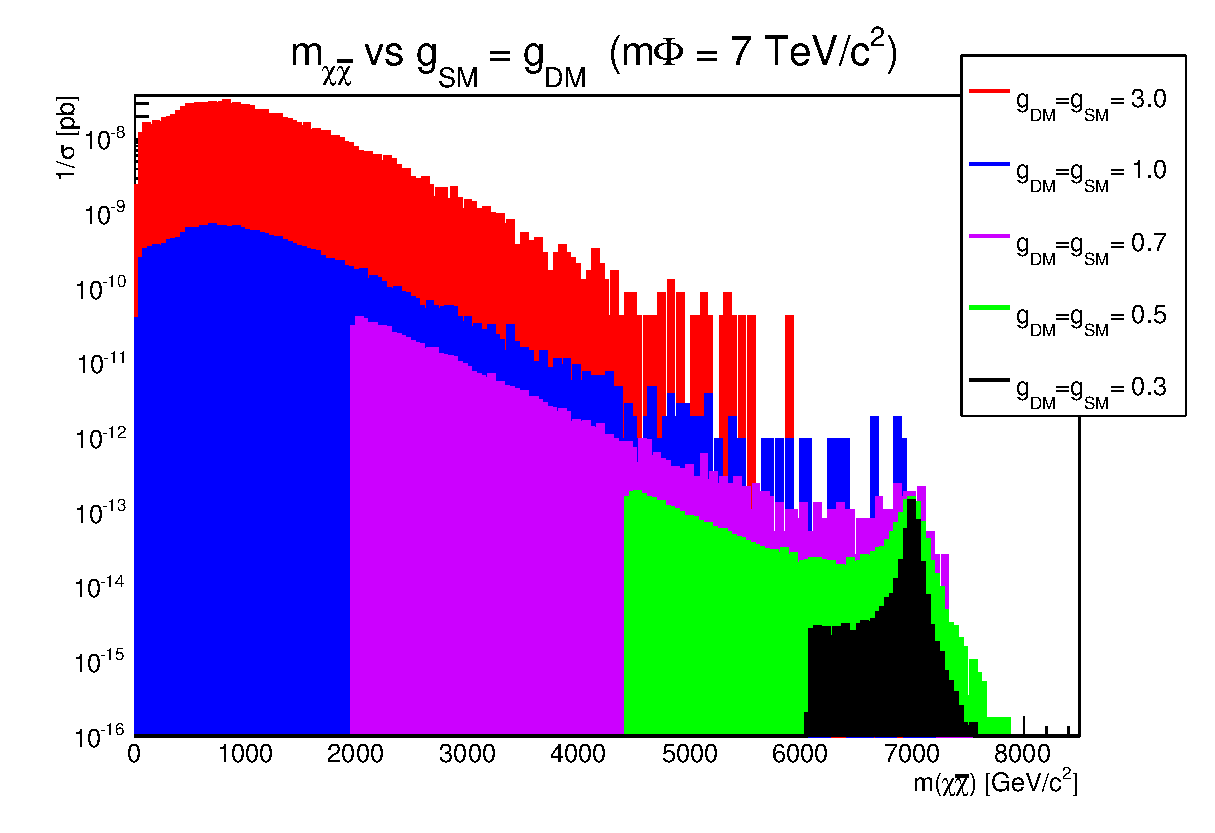
\includegraphics[width=0.9\textwidth]{figures/monojet/mphi_vs_g_xsecwgt_7tev.eps}
\caption{Invariant mass of the Dark Matter pair in the samples with $\mMed=7$~\tev and different coupling strengths.}
\label{fig:monojet_mchichi}
\end{figure}

Since kinematic distributions are robust to
changes in the specific values of coupling, the choice of  \gq=\gDM is reasonable 
to reduce the parameter space to be scanned. 
There are no complications associated
with small couplings, but, also, the early part of Run~2 will not be
sensitive to them.  The range of couplings we recommend limit the
calculated width of the mediator to be near or below \mMed.

For direct mediator searches, asymmetric couplings ($\gq \ne \gDM$ )
might also be considered. A scan in \gDM vs \gq can then be performed for a fixed mediator mass. Such searches, such as those for
dijet resonances, may restrict \gq to a greater degree than
\gDM.

\paragraph{Scan over the Dark Matter mass}

For a fixed mediator mass \mMed and couplings, both the cross section and the kinematic distributions remain similar for different Dark Matter masses as long as $\mMed>2\mDM$.
This simply reflects the fact that most mediators are produced on-shell, and the details of the invisible decay are unimportant.
This is illustrated in Fig.\,\ref{fig:monojet_scan_V_mDM1000} for
an example of \mMed=1~\tev 10~\gev $<\mDM<$ 300~\gev.
It is observed that the cross section decreases as the \mDM approaches $\mMed/2$. Once the Dark Matter pair is produced off-shell, the cross section of the
simplified model is suppressed and the $\MET$ spectrum hardens, as demonstrated with the choice of \mDM=1~\tev in the same plot. Figure\,\ref{fig:monojet_scan_V_mDM100} reveals the $\MET$ spectrum hardens further with increasing \mDM, accompanied by the gradual decrease of the cross section. From these observations one can conclude:
\begin{itemize}
\item A coarse binning along $\mDM$ is sufficient at $\mMed \gg 2\mDM$.
\item Finer binning is needed in order to capture the changes in the cross section and kinematic quantities close to the production threshold on both sides around $\mMed=2\mDM$.
\item Due to the significant cross section suppression of the off-shell Dark Matter pair production, it is not necessary to populate the parameter space $\mMed \ll 2\mDM$ since imminent LHC searches are not expected to be sensitive to these signals.
\end{itemize}

\begin{figure}
\centering
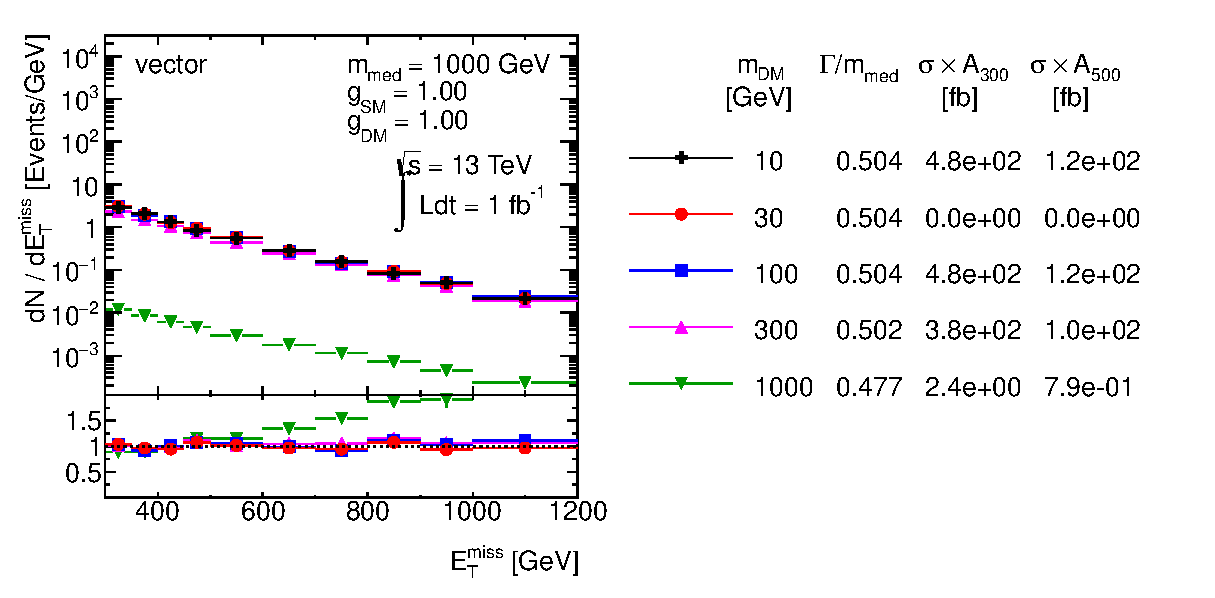
\includegraphics[width=0.9\textwidth]{figures/monojet/scan_mDM_V_1000.eps}
\caption{Scan over Dark Matter mass. The $\MET$ distribution is compared for the vector mediator models using the parameters as indicated. Ratios of the normalized distributions with respect to the first one are shown. $A_{300}$ and $A_{500}$ in the table denote the acceptance of the $\MET>300$~\gev and $\MET>500$~\gev cut, respectively.}
\label{fig:monojet_scan_V_mDM1000}
\end{figure}

\begin{figure}
\centering
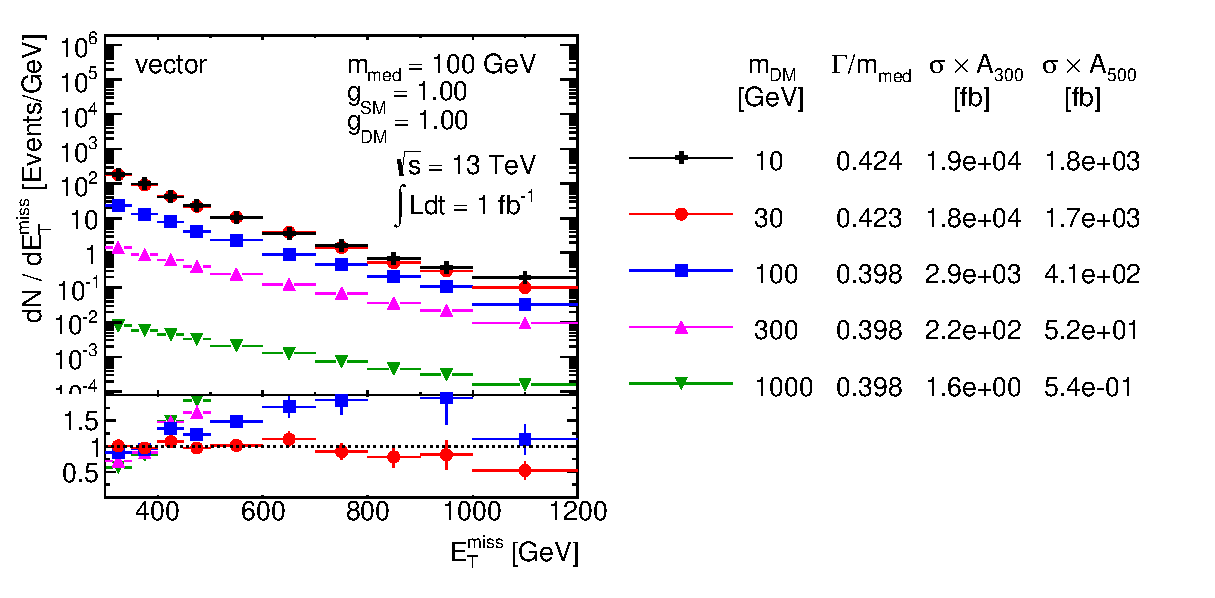
\includegraphics[width=0.9\textwidth]{figures/monojet/scan_mDM_V_100.eps}
\caption{Scan over Dark Matter mass. The $\MET$ distribution is compared for the vector mediator models using the parameters as indicated. Ratios of the normalized distributions with respect to the first one are shown. $A_{300}$ and $A_{500}$ in the table denote the acceptance of the $\MET>300$~\gev and $\MET>500$~\gev cut, respectively.}
\label{fig:monojet_scan_V_mDM100}
\end{figure}


\paragraph{Scan over the mediator mass}

Changing the mediator mass for fixed Dark Matter mass and couplings leads to significant differences in cross section and shapes of the kinematic variables for $\mMed>2\mDM$ as shown in Fig.\,\ref{fig:monojet_scan_V_mMed10}. As expected, higher mediator masses lead to harder $\MET$ spectra.
On the other hand, the $\MET$ shapes are similar in the off-shell Dark Matter production regime.  This
is illustrated in Fig.\,\ref{fig:monojet_scan_V_mMed1000}. Therefore, a coarse binning in $\mDM$ is sufficient at $\mMed \ll 2\mDM$.

\begin{figure}
\centering
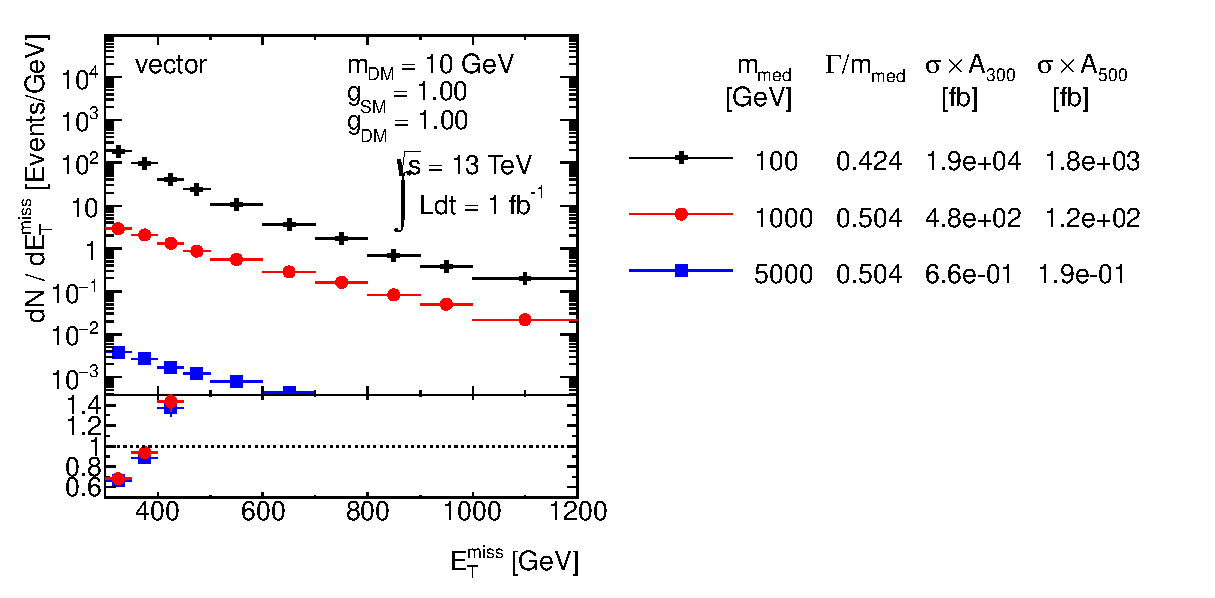
\includegraphics[width=0.9\textwidth]{figures/monojet/scan_mMed_V_10.eps}
\caption{Scan over mediator mass. The $\MET$ distribution is compared for the vector mediator models using the parameters as indicated. Ratios of the normalized distributions with respect to the first one are shown. $A_{300}$ and $A_{500}$ in the table denote the acceptance of the $\MET>300$~\gev and $\MET>500$~\gev cut, respectively.}
\label{fig:monojet_scan_V_mMed10}
\end{figure}

\begin{figure}
\centering
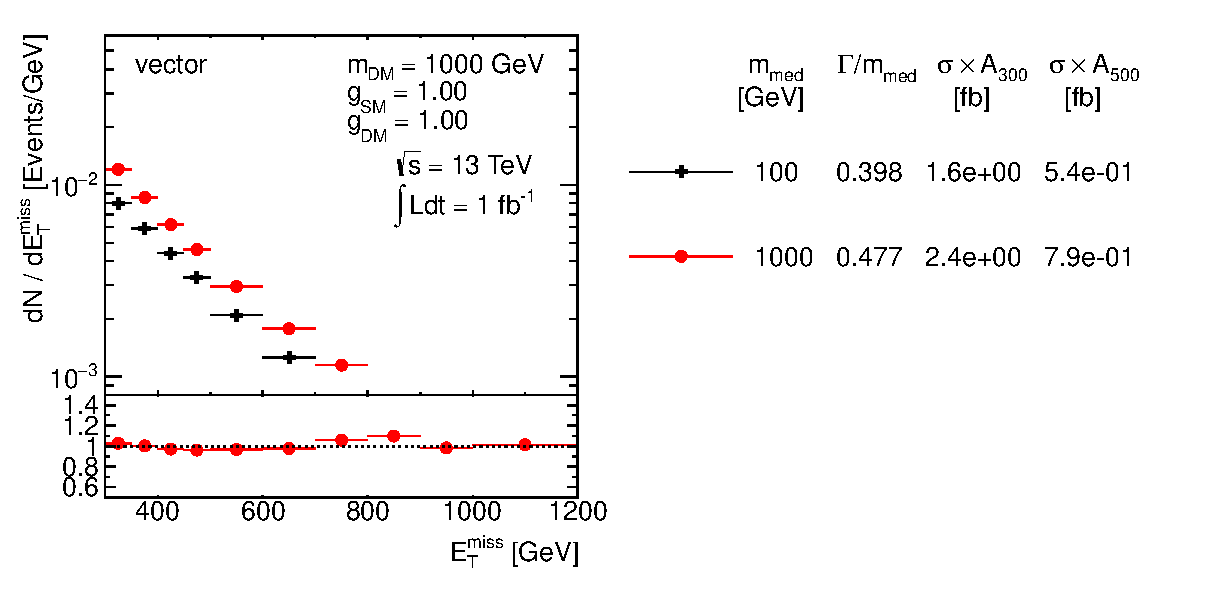
\includegraphics[width=0.9\textwidth]{figures/monojet/scan_mMed_V_1000.eps}
\caption{Scan over mediator mass. The $\MET$ distribution is compared for the vector mediator models using the parameters as indicated. Ratios of the normalized distributions with respect to the first one are shown. $A_{300}$ and $A_{500}$ in the table denote the acceptance of the $\MET>300$~\gev and $\MET>500$~\gev cut, respectively.}
\label{fig:monojet_scan_V_mMed1000}
\end{figure}



\paragraph{Proposed parameter grid}

The final step in proposing a parameter grid is to evaluate the sensitivity
of Run-2 LHC data with respect to rate and/or kinematics.
%In order to motivate the highest mediator mass grid point, the expected sensitivity of Run-2 LHC data needs to be taken into account.
Projected sensitivities for a 14~\tev\, mono-jet analysis are available from ATLAS~\cite{ATL-PHYS-PUB-2014-007}. The expected upper limit at 95\% confidence level on the product of cross section, acceptance and efficiency, $\sigma\times A\times\epsilon$, in the final Run-1 ATLAS mono-jet analysis\,\cite{Aad:2015zva} is 51\,fb and 7.2\,fb  for $\MET>300$~\gev and $\MET>500$~\gev, respectively. ATLAS estimates a factor of two increase in sensitivity with the 2015 data. Given that cross section for $V+$jets processes increases by roughly a factor 2 %\Todo{Can we get more precise number and a citation? Is this in Sarah's V+jets paper?} 
when going from $\sqrt{s}=8$~\tev to 13~\tev, similar fiducial cross section limits can be expected with the first Run-2 data as from the final Run-1 analysis.
The generator level cross section times the acceptance at $\MET>500$~\gev for the model with couplings $\gq=\gDM=1$, a light Dark Matter particle of
\mDM=10~\gev and a \mMed=1~\tev vector mediator is at the order of 100\,fb, i.e. the early Run-2 mono-jet analysis is going to be sensitive to heavier mediators than this. The value of $\sigma\times A$ at $\MET>500$~\gev for 5~\tev vector mediator is at the order of 0.1\,fb, therefore this model probably lies beyond the reach of the LHC in the early Run 2.


Based on these arguments, the following $\mMed$ grid points are chosen, roughly equidistant in the logarithmic scale: 10~\gev, 20~\gev, 50~\gev,  100~\gev, 200~\gev, 300~\gev, 500~\gev, 1000~\gev and 2000~\gev. Given the fact that significant changes in cross section happen around the $\mMed=2\mDM$ threshold, the $\mDM$ grid points are taken at approximately $\mMed/2$, namely: 10~\gev, 50~\gev, 150~\gev, 500~\gev and 1000~\gev. Points on the on-shell diagonal are always chosen to be 5~\gev away from the threshold, 
to avoid numerical instabilities in the event generation. 
The detailed studies of the impact of the parameter changes on the cross section and kinematic distributions presented earlier in this section support removing some of the grid points and relying on interpolation. The optimized grids proposed for the vector and axial-vector mediators are given in Table.\,\ref{tab:mDMmMedScan_VA}, containing 35
%29 
mass points each. One point at very high mediator mass (5~\tev) is added for each of the DM masses scanned, to aid the reinterpretation of results in terms of contact interaction operators (EFTs) as discussed in Section~\ref{sec:RecommendationEFTResults}. 

% \begin{figure}
% \centering
% 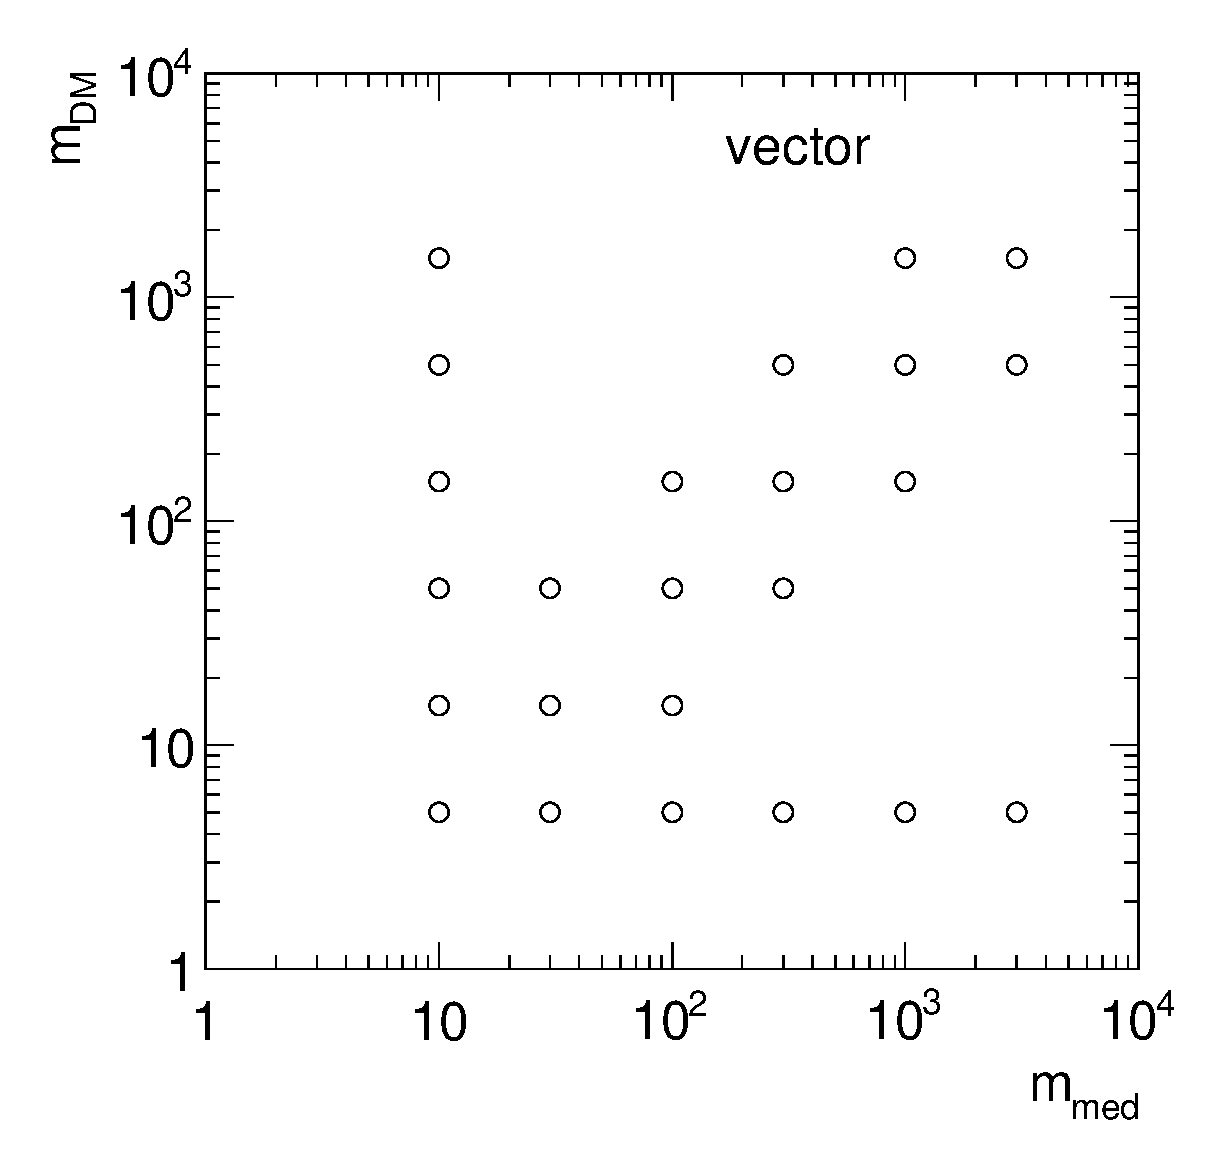
\includegraphics[width=0.45\textwidth]{figures/monojet/grid_V.eps}
% 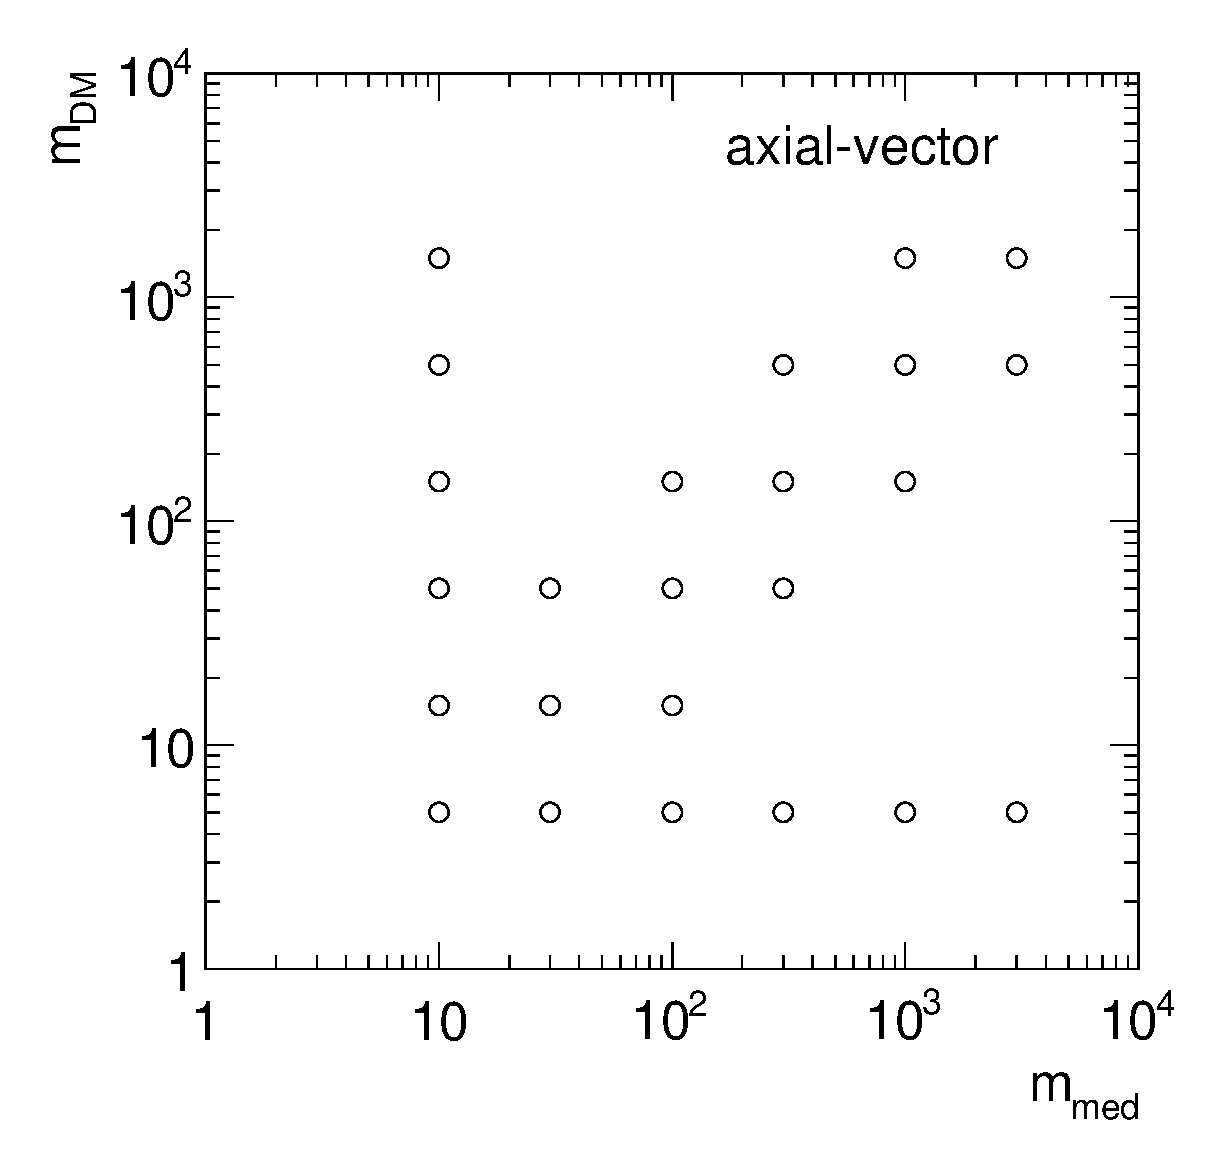
\includegraphics[width=0.45\textwidth]{figures/monojet/grid_A.eps}
% \caption{Proposed parameter grid for vector and axial-vector mediator in the $\mMed$--$\mDM$ plane.}
% \label{fig:monojet_grid_V}
% \end{figure}

\begin{table}[!h]
\centering
\resizebox{\textwidth}{!}{
\begin{tabular}{| l |r r r r r r r r r r|}
\hline
\multicolumn{1}{|c|}{\mDM/\gev} & \multicolumn{10}{c|}{\mmed/\gev} \\
\hline
 1             &         10  & 20 & 50 & 100 & 200 & 300 & 500 &         1000  &                 2000   &         5000  \\
 10   	       &         10  & 15 & 50 & 100 &     &     &     &               &                        &     5000      \\
 50            &   10  & 
& 50 &  95 & 200 & 300 &     &               &                        &    5000       \\
 150           &         10  &    &    &     & 200 & 295 & 500 &        & 1000                 &     5000      \\
 500           &         10  &    &    &     &     &     & 500 &          995  &                 2000   &     5000      \\
 1000          &         10  &    &    &     &     &     &     &         1000  &                 1995   &         5000  \\
\hline
\end{tabular}
}
\caption{Simplified model benchmarks for $s-$channel simplified models (spin-1 mediators 
decaying to Dirac DM fermions in the V and A case, taking the minimum width for \gq = \gDM = 1)}.
% Points in \textbf{bold} are only generated for the vector/axial vector cases, while points in 
% \textit{italics} are generated for the monojet analysis 
% but not for the search including heavy quarks. This table corresponds to 29 points for monojet vector/axial vector models,
% 26 points for monojet scalar/pseudoscalar models and 24 points for $t \bar{t}$+\MET scalar/pseudoscalar models.}

\label{tab:mDMmMedScan_VA}
% \end{sidewaystable}
\end{table}

The presentation of the results in the $\gq$--$\gDM$ plane for fixed masses benefits from cross section scaling and is discussed in Section\,\ref{sec:monojet_scaling}.

%% It is difficult to visualize a four dimensional scan.
%% However, it is convenient to study the parameter dependence,
%% and present results, in two projections:
%% (a) the $\mMed$--$\mDM$ plane for a particular choice of the couplings, and\\
%% (b) the $\gq$--$\gDM$ plane for a particular choice of the masses.

%% %discuss expected sensitivity (cite PUB note) when motivating mDM and mMed range
%% %motivate the mass point for the coupilng scan

%% We choose to display the results in the $\mMed$--$\mDM$ plane for the choice of the couplings $\gq=\gDM=1$. 



\section{Scalar and pseudoscalar mediator, \schannel exchange}
\label{sec:monojet_scalar}

\begin{figure}
\centering
\unitlength=0.005\linewidth
	\subfloat[\label{subfig:modelMonoHbaryonicggS}]	{
	\begin{feynmandiagram}[appendixmodelSmonojetTopTriangle]
		\fmfleft{i1,i2}
		\fmfright{o1,o2}
		\fmftop{isr}
		\fmfbottom{pisr}
		\fmfpolyn{empty}{v}{3}
		\fmf{fermion}{i2,v6}
		\fmf{phantom}{i1,pv1,v1}
		\fmf{gluon,tension=0}{i1,v1}
		\fmf{gluon}{v6,v3}
		\fmf{dashes,label={\LARGE $S,,P$}}{v2,v5}
		\fmf{fermion,tension=1.2}{o2,v5,o1}
		\fmfdot{v1,v6,v2,v3,v5}
		\fmffreeze
		\fmf{phantom}{pv1,pisr}
		\fmf{fermion}{v6,isr}
		\fmflabel{\LARGE ${g}$}{i1}
		\fmflabel{\LARGE ${q}$}{i2}
		\fmflabel{\LARGE ${q}$}{isr}
		\fmflabel{\LARGE $\bar\chi$}{o1}
		\fmflabel{\LARGE $\chi$}{o2}
	\end{feynmandiagram}
}


	\subfloat[\label{subfig:modelMonoHbaryonicggS}]	{
	\begin{feynmandiagram}[appendixmodelSmonojetTopBox]
		\fmfleft{i1,i2}
		\fmfright{o1,o2,hisr,isr}
		\fmfpolyn{empty}{v}{4}
		\fmf{gluon}{i2,v4}
		\fmf{gluon}{i1,v1}
		\fmf{dashes,label={\LARGE $S,,P$}}{v2,vwimp}
		\fmflabel{\LARGE ${g}$}{i1}
		\fmflabel{\LARGE ${g}$}{i2}
		\fmflabel{\LARGE ${g}$}{isr}
		\fmflabel{\LARGE $\bar\chi$}{o1}
		\fmflabel{\LARGE $\chi$}{o2}
		\fmf{fermion}{o2,vwimp,o1}
		\fmfdot{v1,v2,v3,v4,vwimp}
		\fmf{gluon}{v3,isr}
	\end{feynmandiagram}
}
\setfloatalignment{t}
\vspace{0.5\baselineskip}
	\caption
	{
		One-loop diagrams of processes exchanging a scalar ($S$) or pseudoscalar ($P$) mediator, leading to a mono-jet signature. 
	}
	\label{fig:feyn_prod_S}
\end{figure}

In this section, we consider a parallel situation to the \modelDMV and \modelDMA mediators in the previous sections: a real scalar or a pseudoscalar where the associated scalar is decoupled at higher energies\sidenote{This assumption does not hold in a UV-complete model where the two components of the complex scalar mediator would be approximately degenerate.  The complex scalar case could be studied separately in the case of heavy flavor final states given the sufficiently different kinematics.}. This section is largely based on Refs.~\cite{Buckley:2014fba,Harris:2014hga} which contain a thorough discussion of these models. 

Under MFV, spin-$0$ resonances look like an alternate-reality version of the SM Higgs. Relative to the \modelDMV and \modelDMA discussed above, these \modelDMS and \modelDMP models are distinguished by the special consequences of the MFV assumption, the very narrow width of the mediator and its extreme sensitivity to which decays are kinematically availabile, and the loop-induced coupling to gluons. The interaction Lagrangians are

 \begin{eqnarray}
{\cal L}_{\phi} & = &
%{\cal L}_{\rm SM}+i\bar{\chiDM} \slashed{\partial} \chiDM + m_\chiDM \bar{\chiDM}\chiDM + \left| \partial_\mu \phi \right|^2+\frac{1}{2}m_\phi^2 \phi^2 + \nonumber \\ 
%& &
g_\chiDM \phi \bar{\chiDM}\chiDM+ \frac{\phi}{\sqrt{2}} \sum_i \left(g_u y_i^u \bar{u}_i u_i+g_d y_i^d \bar{d}_i d_i+g_\ell y_i^\ell \bar{\ell}_i \ell_i\right)\, , \label{eq:scalarlag} \\
{\cal L}_{a} & = &
%{\cal L}_{\rm SM}+i\bar{\chiDM} \slashed{\partial} \chiDM + m_\chiDM \bar{\chiDM}\chiDM + \left| \partial_\mu a \right|^2+\frac{1}{2}m_a^2 a^2 + \nonumber \\
%& &
ig_\chiDM a \bar{\chiDM}\gamma_5\chiDM+ \frac{i a}{\sqrt{2}}\sum_i  \left(g_u y_i^u \bar{u}_i \gamma_5 u_i+g_d y_i^d \bar{d}_i \gamma_5 d_i+ \right. \nonumber \\
& & \left. g_\ell y_i^\ell   \bar{\ell}_i \gamma_5 \ell_i\right) \,. \label{eq:pseudoscalarlag}
\end{eqnarray}
where the Yukawa couplings $y_i^f$ are normalized to the Higgs vev as $y_i^f = \sqrt{2}m_i^f/v$. 

The couplings to fermions are proportional to the SM Higgs couplings, yet one is still allowed to adjust an overall strength of the coupling to charged leptons and the relative couplings of $u$- and $d$-type quarks. As in the preceding sections, for the sake of simplicity and straightforward comparision, we reduce the couplings to the SM fermions to a single universal parameter $g_v \equiv g_u = g_d = g_\ell$  \sidenote{The contribution from $\tau^+\tau^-$ decays plays no role for most of the parameter space considered.}. In this framework on can compare the relative discovery and exclusion power of each search, though again we emphasize the importance of searching the full set of allowed channels in case violations of these simplifying assumptions lead to signficant modifications of the decay rates which unexpectedly favor different channels than the mix obtained under our assumptions. The coupling $g_\chiDM$ parameterises the entire dependence on the structure between the mediator and the dark sector.

%The most general Lagrangians including new scalars or pseudoscalars will have a potential containing interactions with the SM Higgs field $h$. 
 %If there is no indication otherwise the easiest assumptions is always the most scientific to chose (also listening to some phenomenologists this seems not always to be the case ;-) )  

Given these simplifications, the minimal set of parameters under consideration is
 \bea
  \left\{ m_\chiDM,~ m_{\phi/a},~ g_\chiDM,~ g_v \right\} \,.
 \eea

Fig.~\ref{fig:feyn_prod_S} shows the one-loop diagrams producing a \MET+X signature.

%The simplest choice of couplings, known as Minimal Simplified Dark Matter model (MSDM) \textbf{[TODO: add references]}, is $g_u = g_d = g_\ell$, which is realized in singlet scalar extensions of the SM. 

% Despite our simplifying assumption, one should keep the more general possibility in mind, as even simple extensions of the mediating sector can result in $g_u \neq g_d \neq g_\ell$. A well-known realization of this would be the coupling of the pseudoscalar to up-type quarks (proportional to $m_u \cot\beta$) and down-type quarks and charged leptons (proportional to $m_{d/\ell}\tan\beta$) in two-Higgs doublet extensions of the SM. Here $\tan \beta$ denoting the ratio of vacuum expectation values of the two Higgs doublets. %The case $g_u \neq  g_d \neq g_\ell$ requires additional scalars with potentially large masses. 
% This possibility of non-equal couplings motivates searches in complementary channels which probe couplings to different flavors of quarks and leptons.

%Extending the SM Higgs sector to a two Higgs doublet model implies more complex couplings such as  $g_u = \cot \beta$ and $g_d = g_e = \tan \beta$ where $\tan \beta$ denotes the ratio of vacuum expectation values of the two Higgs doublets.  The case $g_u \neq  g_d \neq g_\ell$ requires more additional scalars with potentially large masses, and it is not covered here: for simplicity, we assume universal SM-mediator couplings $g_v = g_u = g_d = g_\ell$ in the remainder of this work. 


%The model assumes Dirac Dark Matter particles and is based on the minimal flavor violation (MFV), which motivates Higgs-like Yukawa couplings of the mediator to the Standard Model quarks. No other couplings, such as to leptons, are allowed in this model.
%The following two cases are considered:\\
%(a) scalar couplings to DM and SM,\\
%(b) pseudo-scalar couplings to DM and SM\\
%\noindent with the corresponding Lagrangians written as:
%\begin{align}
%\label{eq:SP} 
%\mathcal{L}_{\mathrm{scalar}} &= \gq \sum \frac{m_q}{v} (\bar{q}q) S + \gDM (\bar{\chiDM}\chiDM) S \\
%\mathcal{L}_{\mathrm{pseudo-scalar}} &= \gq \sum \frac{m_q}{v} (\bar{q}\gamma^5q) P + \gDM (\bar{\chiDM}\gamma^5\chiDM) P \\
%\end{align}
%where $v=246$~\gev denotes the Higgs vacuum expectation value.

The minimal mediator width is given by %Eq.\,\ref{eq:monojet_min},
\begin{fullwidth}
  \begin{equation} \label{eq:width}
    \begin{split}
      \Gamma_{\phi,a} = & \sum_f N_c \frac{y_f^2 g_v^2 m_{\phi,a}}{16
        \pi} \left(1-\frac{4 m_f^2}{m_{\phi,a}^2}\right)^{x/2}
      + \frac{g_\chiDM^2 m_{\phi,a}}{8 \pi} \left(1-\frac{4 m_\chiDM^2}{m_{\phi,a}^2}\right)^{x/2}\\
      & + \frac{\alpha_s^2 y_t^2 g_v^2 m_{\phi,a}^3}{32 \pi^3 v^2}
      \left| f_{\phi,a}\left(\tfrac{4m_t^2}{m_{\phi,a}^2}
        \right)\right|^2
    \end{split}
  \end{equation}
\end{fullwidth}
where $x=3$ for scalars and $x=1$ for pseudoscalars. The loop integrals are

\begin{fullwidth}
  \bea \label{eq:fphifa}
  f_\phi (\tau) &=& \tau \left [ 1+ (1-\tau) \arctan^2 \left ( \frac{1}{\sqrt{\tau-1}} \right ) \right ]  \,, \\
  f_a (\tau) &=& \tau \arctan^2 \left ( \frac{1}{\sqrt{\tau-1}}
  \right) \, 
  \eea
\end{fullwidth}
 where $\tau = 4 m_{t}^2/m_{\phi,a}^2$, and, for $\tau > 1$, 
\begin{fullwidth}
  \bea \label{eq:fphifb}
  f_\phi (\tau) &=& \tau \left [ 1+ (1-\tau)\left(-\frac{1}{4}\left(\log\frac{1+\sqrt{1-\tau}}{1-\sqrt{1-\tau}}+i\pi\right)^2\right) \right ]  \,\,,\\
  f_a (\tau) &=& \tau
  \left(-\frac{1}{4}\left(\log\frac{1+\sqrt{1-\tau}}{1-\sqrt{1-\tau}}+i\pi\right)^2\right).
  \eea
\end{fullwidth}

% If this is in the DM@LHC write-up, it is unnecessary here.
% The first term in the width corresponds to the decay into SM fermions, and the sum runs over all kinematically available fermions, $N_c = 3$ for quarks. The second term is the decay into DM, assuming that is kinematically allowed. The factor of two between the decay into SM  fermions and into DM  is a result of our choice of normalization of the Yukawa couplings due to spin dependencies. The last term corresponds to decay into gluons.  Since we have assumed that $\gq = g_u = g_d = g_\ell$, we have included in the partial decay widths $\Gamma (\phi/a \to gg)$ only the contributions stemming from top loops, which provide the by far largest corrections given that $y_t \gg y_b$~etc. At the loop level the mediators can decay not only to gluons but also to pairs of photons and other final states if kinematical accessible. However the decay rates $\Gamma (\phi/a \to gg)$ are always larger than the other loop-induced partial widths, and in consequence the total decay widths $\Gamma_{\phi/a}$ are well approximated by the corresponding sum of the individual partial decay widths involving DM, fermion or gluon pairs. It should be noted that if  $m_{\phi/a} > 2m_t$ the total widths of $\phi/a$ will typically be dominated by the partial widths to top quarks.


%\begin{equation}
%\Gamma_{\rm{min}}^{S/P}=\Gamma_{\bar{\chiDM}\chiDM}^{S/P} + \sum_{q}\Gamma_{\bar{q}q}^{S/P} + \Gamma_{gg}^{S/P},
%\end{equation}
%with the following LO expressions for the partial widths:
%\begin{align}
%\Gamma_{\bar{\chiDM}\chiDM}^{\rm{S}}&=\frac{\gDM^2 \mMed}{8\pi}\beta_{DM}^{3/2} \theta(\mMed-2\mDM)\\
%\Gamma_{\bar{q}q}^{\rm{S}}&= \frac{3 \gq^2 \mMed}{8\pi}\frac{m_q^2}{v^2}\beta_q^{3/2} \theta(\mMed-2m_q)\\
%\Gamma_{gg}^{\rm{S}}&= \frac{\gq^2 \alpha_s^2}{2\pi^3 v^2 \mMed} \left| \sum_q m_q^2 F_{\rm{S}} \left( \frac{4m_q^2}{\mMed^2} \right) \right|^2\\
%\Gamma_{\bar{\chiDM}\chiDM}^{\rm{P}}&=\frac{\gDM^2 \mMed}{8\pi} \beta_{DM}\theta(\mMed-2\mDM)\\
%\Gamma_{\bar{q}q}^{\rm{P}}&= \frac{3 \gq^2 \mMed}{8\pi}\frac{m_q^2}{v^2}\beta_{q}\theta(\mMed-2m_q)\\
%\Gamma_{gg}^{\rm{P}}&= \frac{\gq^2 \alpha_s^2}{2\pi^3 v^2 \mMed} \left| \sum_q m_q^2 F_{\rm{P}} \left( \frac{4m_q^2}{\mMed^2} \right) \right|^2\;,
%\label{eq:GammaS}
%\end{align}
%with the form factors defined as
%\begin{align}
%F_{\rm{S}}(x)&= 1+(1-x)\arctan^2\left(\frac{1}{\sqrt{x-1}}\right)\\
%F_{\rm{P}}(x)&= \arctan^2\left(\frac{1}{\sqrt{x-1}}\right)\;.
%\end{align}

%%Start Matt Buckley's edits 
%\begin{equation} \label{eq:width}
%\begin{split}
%\Gamma_{\phi,a}  = & \sum_f N_c \frac{y_f^2 g_v^2 m_{\phi,a}}{16 \pi} \left(1-\frac{4 m_f^2}{m_{\phi,a}^2}\right)^{x/2}
%+ \frac{g_\chiDM^2 m_{\phi,a}}{8 \pi} \left(1-\frac{4 m_\chiDM^2}{m_{\phi,a}^2}\right)^{x/2}\\
%& + \frac{\alpha_s^2 y_t^2 g_v^2 m_{\phi,a}^3}{32 \pi^3 v^2} \left| f_{\phi,a}\left(\tfrac{4m_t^2}{m_{\phi,a}^2} \right)\right|^2
%\end{split}
%\end{equation}
%
%where $x=3$ for scalars and $x=1$ for pseudoscalars, and the loop integrals are
%
%\bea \label{eq:fphifa}
%f_\phi (\tau) = \tau \left [ 1+ (1-\tau) \arctan^2 \left ( \frac{1}{\sqrt{\tau-1}} \right ) \right ]  \,, \qquad 
%f_a (\tau) =  \tau \arctan^2 \left ( \frac{1}{\sqrt{\tau-1}} \right ) \,. 
%\eea
%
%The first term in each width corresponds to the decay into SM fermions (the sum runs over all kinematically available fermions, $N_c = 3$ for quarks and $N_c = 1$ for leptons). The second term is the decay into DM (assuming that this decay is kinematically allowed). The factor of two between the decay into SM  fermions and into DM  is a result of our choice of normalization of the Higgs vacuum expectation value and the Yukawa couplings.
%

%%BP: Is this the best way to express that? I'd add:... due to spin dependencies. 
%%MB: yes. I don't think it's a spin thing, it's just that we've defined v = 246, so the SM fermions get a $1/\sqrt{2}^2$ that DM doesn't.

%The last two terms correspond to decay into gluons.  Since we have assumed that $g_v = g_u = g_d = g_\ell$, we have included in the partial decay widths $\Gamma (\phi/a \to gg)$ only the contributions stemming from top loops, which provide the by far largest corrections given that $y_t \gg y_b$~etc. At the loop level the mediators can decay not only to gluons but also to pairs of photons and other final states if kinematical accessible. However the decay rates $\Gamma (\phi/a \to gg)$ are always larger than the other loop-induced partial widths, and in consequence the total decay widths $\Gamma_{\phi/a}$ are well approximated by the corresponding sum of the individual partial decay widths involving DM, fermion or gluon pairs. It should be noted that if  $m_{\phi/a} > 2m_t$ the total widths of $\phi/a$ will typically be dominated by the partial widths to top quarks.

%%%End Matt Buckley's edits

The minimal widths for scalar and pseudo-scalar mediators with $\gq=\gDM=1$ are shown in Fig.\,\ref{fig:monojet_width_S}, illustrating the effect of choosing
the SM Higgs-like Yukawa couplings for the SM fermions.
For the mediator mass above twice the top quark mass $m_t$, the minimal width receives the dominant contribution from the top quark. For lighter mediator masses, Dark Matter dominates as the couplings to lighter quarks are Yukawa suppressed.
%Note that the partial width coming from gluons through loops can be safely neglected\,\cite{Haisch:2015ioa}.


\begin{figure}
\centering
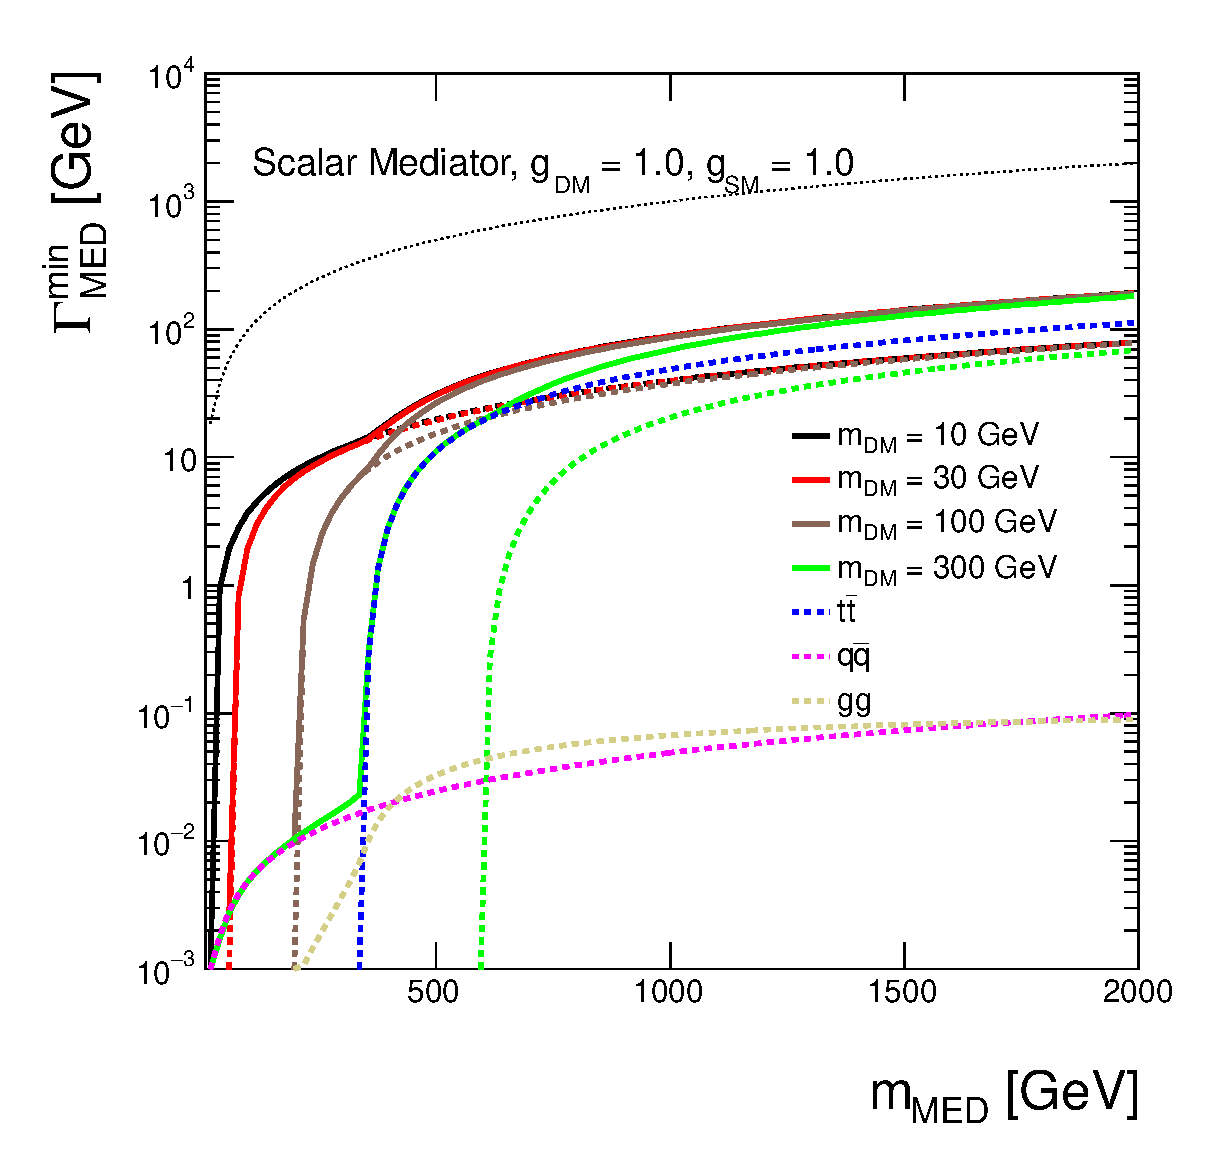
\includegraphics[width=0.45\textwidth]{figures/monojet/width_S.eps}
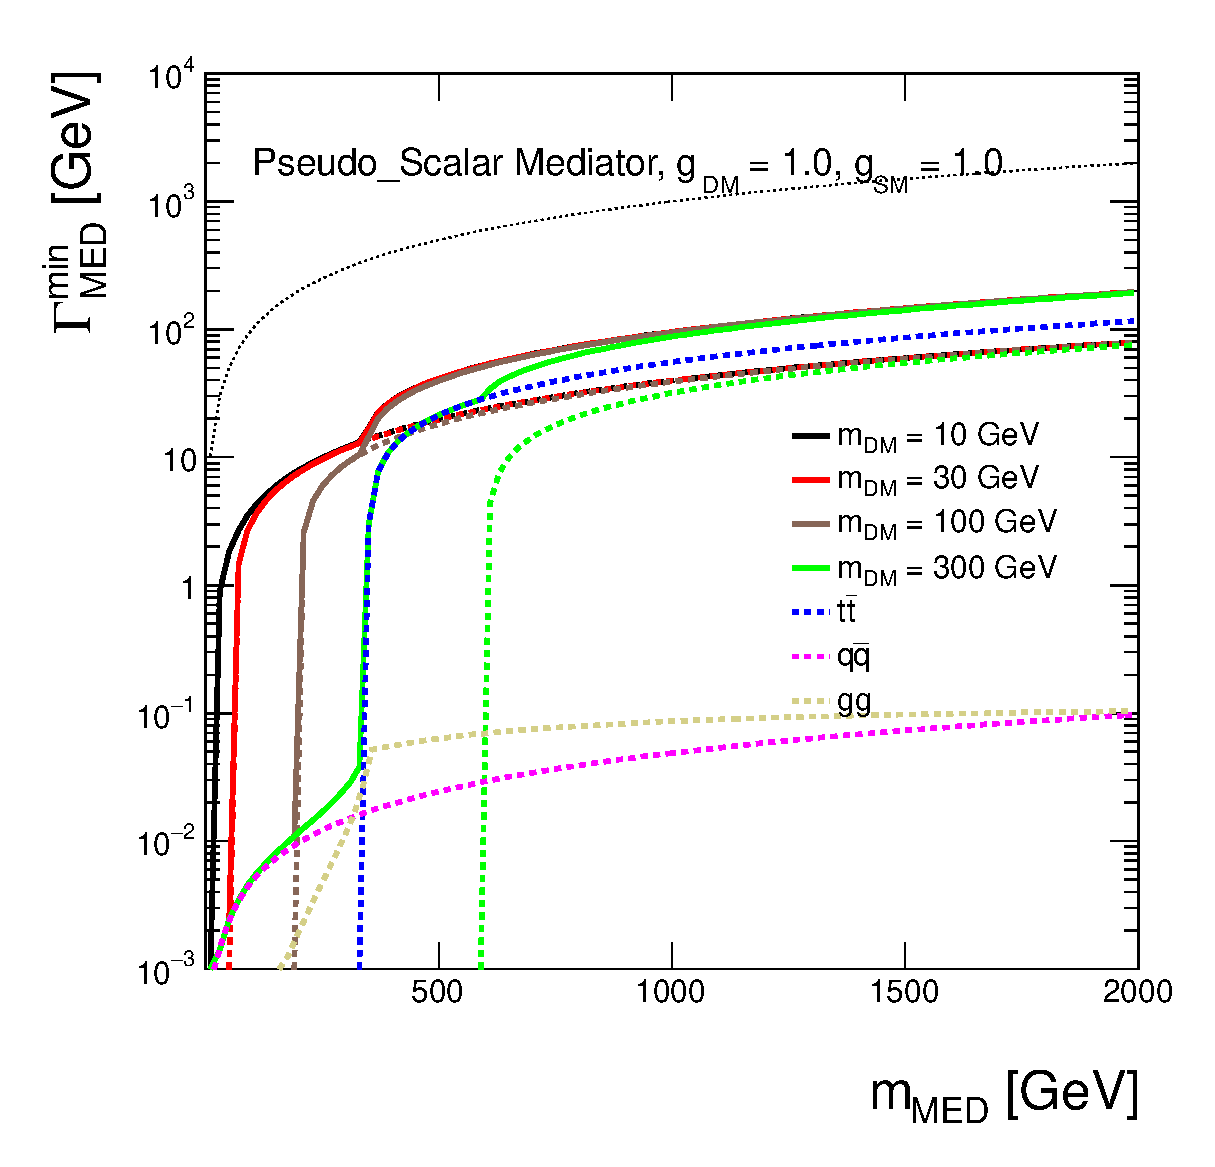
\includegraphics[width=0.45\textwidth]{figures/monojet/width_P.eps}
\caption{Minimal width as a function of mediator mass for scalar and pseudo-scalar mediator assuming couplings of 1. The total width is shown as solid lines for Dark Matter masses of \mDM=10~\gev, 30~\gev, 100~\gev and 300~\gev in black, red, brown and green, respectively. The individual contributions from Dark Matter are indicated by dotted lines with the same colors. The contribution from all quarks but top is shown as magenta dotted line and the contribution from top quarks only is illustrated by the dotted blue line. The dotted beige line shows the contribution fron the coupling to gluons. The dotted black line shows the extreme case $\Gamma_{\rm{min}}=\mMed$.}
\label{fig:monojet_width_S}
\end{figure}

It can be seen in Fig.~\ref{fig:monojet_kinematics_SP} that the kinematics for the scalar and pseudoscalar models coincides.
For this reason, we recommend to only generate only one of the two models, and report the cross-sections on HEPData 
\Todo{Clarify shape of model repository} for the other one. No preference is given between the two models as they have the
same kinematics, although it is worth pointing out that the pseudo-scalar model has been used for a Dark Matter interpretation of the DAMA signal 
and of the galactic center excess~\cite{Arina:2014yna}.

\begin{figure}
	\centering
	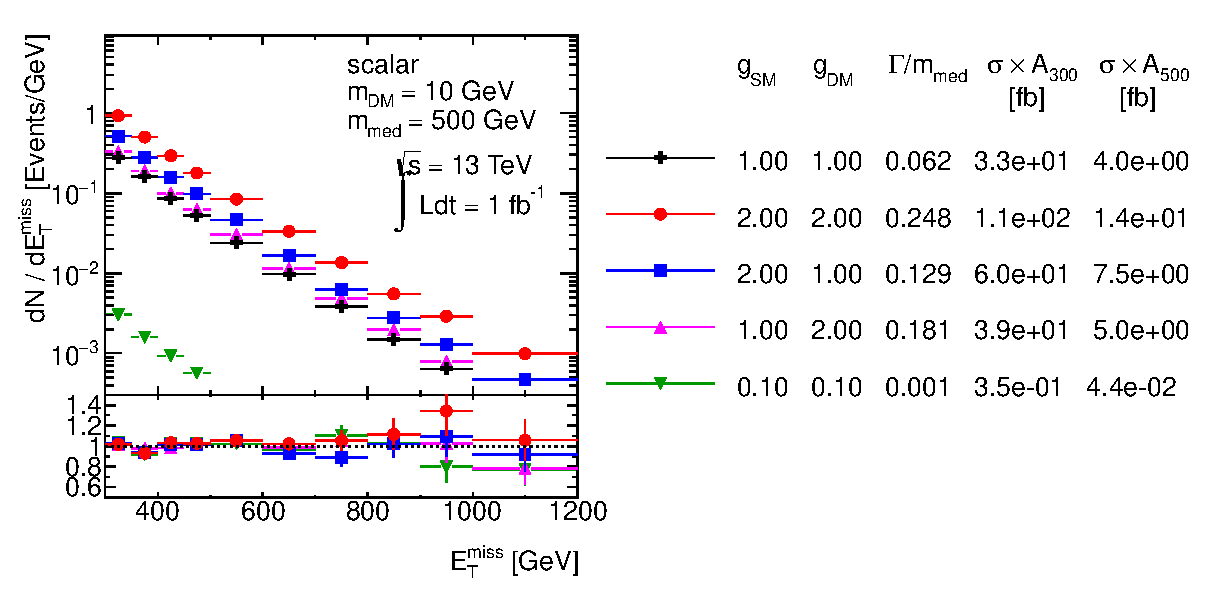
\includegraphics[width=0.9\textwidth]{figures/monojet/scan_g_S_10_500.eps}
	\caption{PLACEHOLDER: Comparison of the $\MET$ distributions for the scalar and pseudoscalar models for different DM and mediator masses. 
	Ratios of the normalized distributions with respect to the first one are shown. $A_{300}$ and $A_{500}$ in the table denote the acceptance of the $\MET>300$~\gev and $\MET>500$~\gev cut, respectively.}
	\label{fig:monojet_kinematics_SP}
\end{figure}

Similarly as in the case of the vector and axial-vector couplings
of spin-1 mediators, scans in the parameter space are performed also for the scalar and pseudo-scalar couplings of the spin-0 mediators
in order to decide on the optimized parameter grid for the presentation of Run-2 results. Figures\,\ref{fig:monojet_scan_S_g}-
%, fig:monojet_scan_S_mDM1000,fig:monojet_scan_S_mDM100, fig:monojet_scan_S_mMed10, 
\ref{fig:monojet_scan_S_mMed1000} show the scans over the couplings, Dark Matter mass and mediator mass and the same conclusions apply as in Section\,\ref{sec:monojet_V}.

%TODO does the discussion below make sense?
A scan over the mediator mass is shown in Fig.\,\ref{fig:monojet_scan_S_mMed1000} where \mMed = 300~\gev and 500~\gev are chosen to be below and above $2m_t$. The off-shell Dark Matter production regime is assumed by taking an extreme limit ($\mDM=1$~\tev) in order to study solely the effects of the couplings to quarks. 
No differences in the kinematic distributions are observed and also the cross sections remain similar in this case. No significant changes appear for mediator masses around the $2m_t$ threshold.

\begin{figure}
\centering
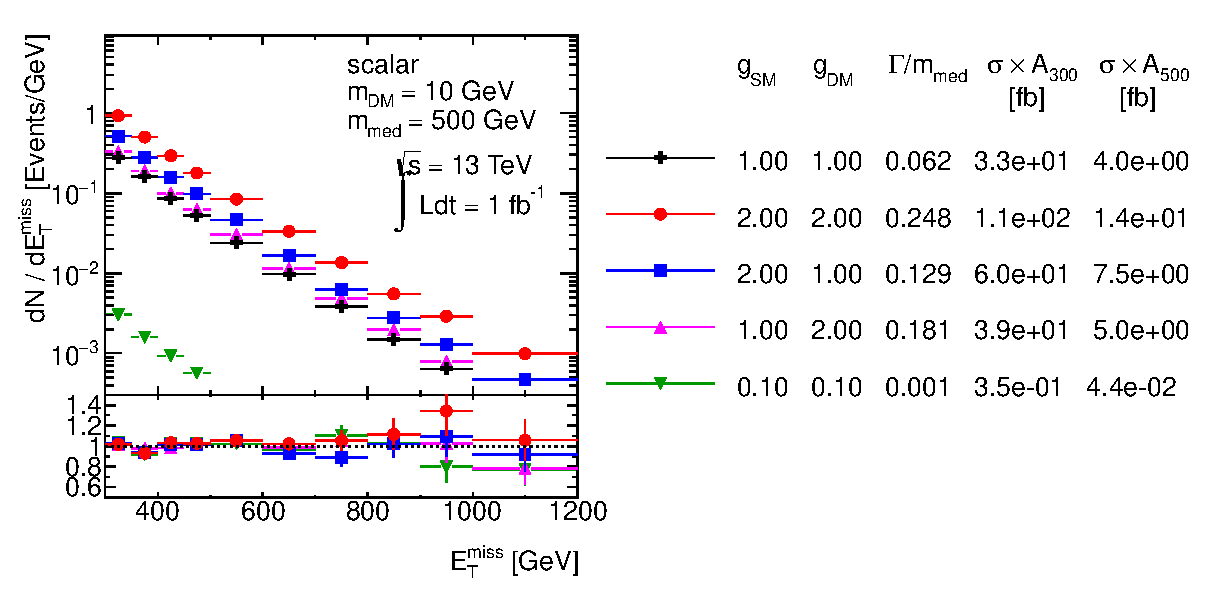
\includegraphics[width=0.9\textwidth]{figures/monojet/scan_g_S_10_500.eps}
\caption{Scan over couplings. The $\MET$ distribution is compared for the scalar mediator models using the parameters as indicated. Ratios of the normalized distributions with respect to the first one are shown. $A_{300}$ and $A_{500}$ in the table denote the acceptance of the $\MET>300$~\gev and $\MET>500$~\gev cut, respectively.}
\label{fig:monojet_scan_S_g}
\end{figure}

\begin{figure}
\centering
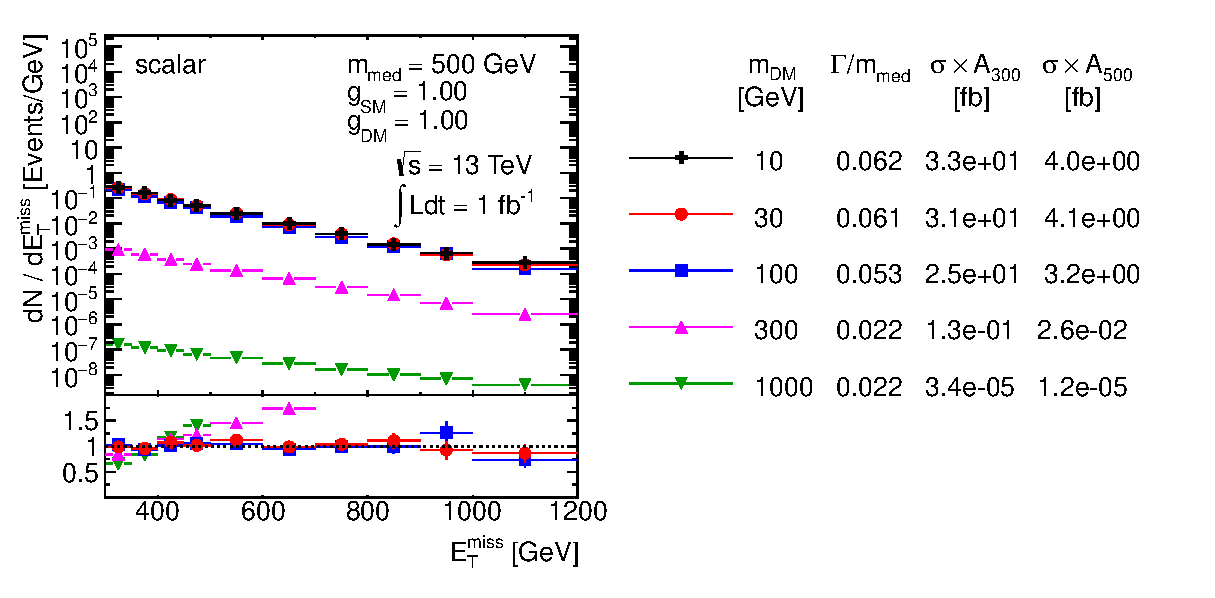
\includegraphics[width=0.9\textwidth]{figures/monojet/scan_mDM_S_500.eps}
\caption{Scan over Dark Matter mass. The $\MET$ distribution is compared for the scalar mediator models using the parameters as indicated. Ratios of the normalized distributions with respect to the first one are shown. $A_{300}$ and $A_{500}$ in the table denote the acceptance of the $\MET>300$~\gev and $\MET>500$~\gev cut, respectively.}
\label{fig:monojet_scan_S_mDM1000}
\end{figure}

\begin{figure}
\centering
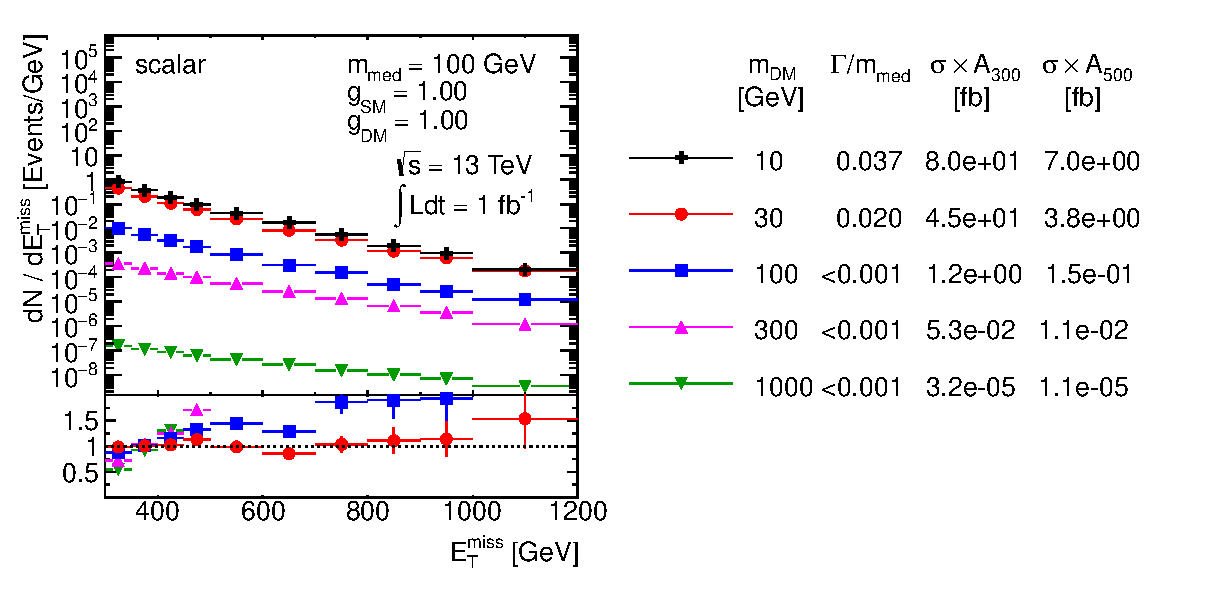
\includegraphics[width=0.9\textwidth]{figures/monojet/scan_mDM_S_100.eps}
\caption{Scan over Dark Matter mass. The $\MET$ distribution is compared for the scalar mediator models using the parameters as indicated. Ratios of the normalized distributions with respect to the first one are shown. $A_{300}$ and $A_{500}$ in the table denote the acceptance of the $\MET>300$~\gev and $\MET>500$~\gev cut, respectively.}
\label{fig:monojet_scan_S_mDM100}
\end{figure}

\begin{figure}
\centering
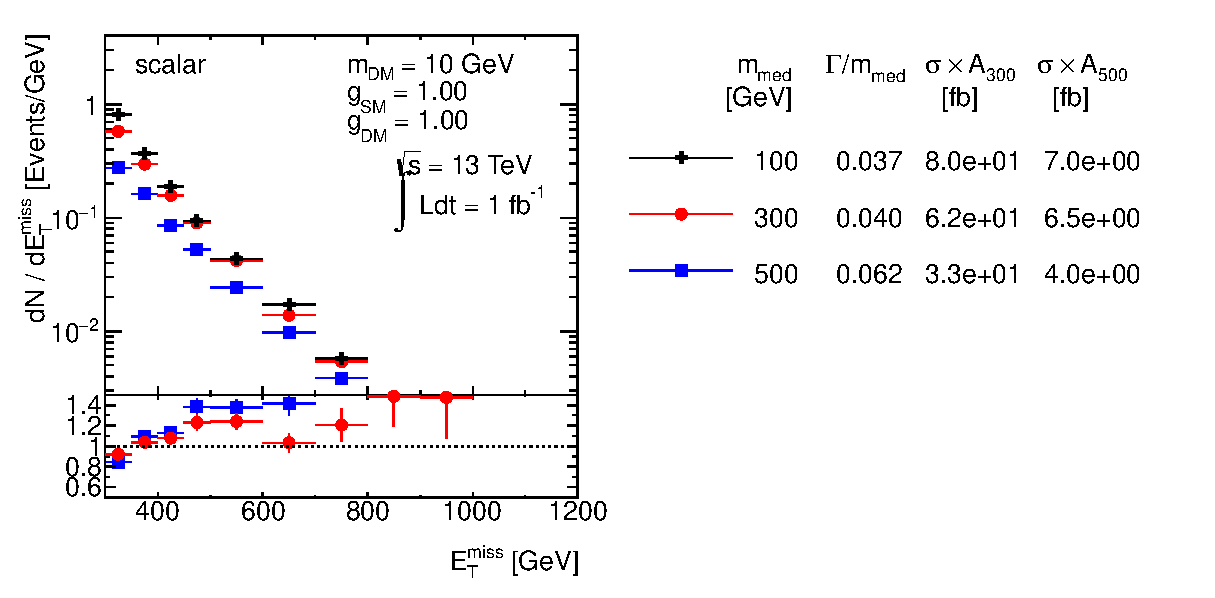
\includegraphics[width=0.9\textwidth]{figures/monojet/scan_mMed_S_10.eps}
\caption{Scan over mediator mass. The $\MET$ distribution is compared for the scalar mediator models using the parameters as indicated. Ratios of the normalized distributions with respect to the first one are shown. $A_{300}$ and $A_{500}$ in the table denote the acceptance of the $\MET>300$~\gev and $\MET>500$~\gev cut, respectively.}
\label{fig:monojet_scan_S_mMed10}
\end{figure}

\begin{figure}
\centering
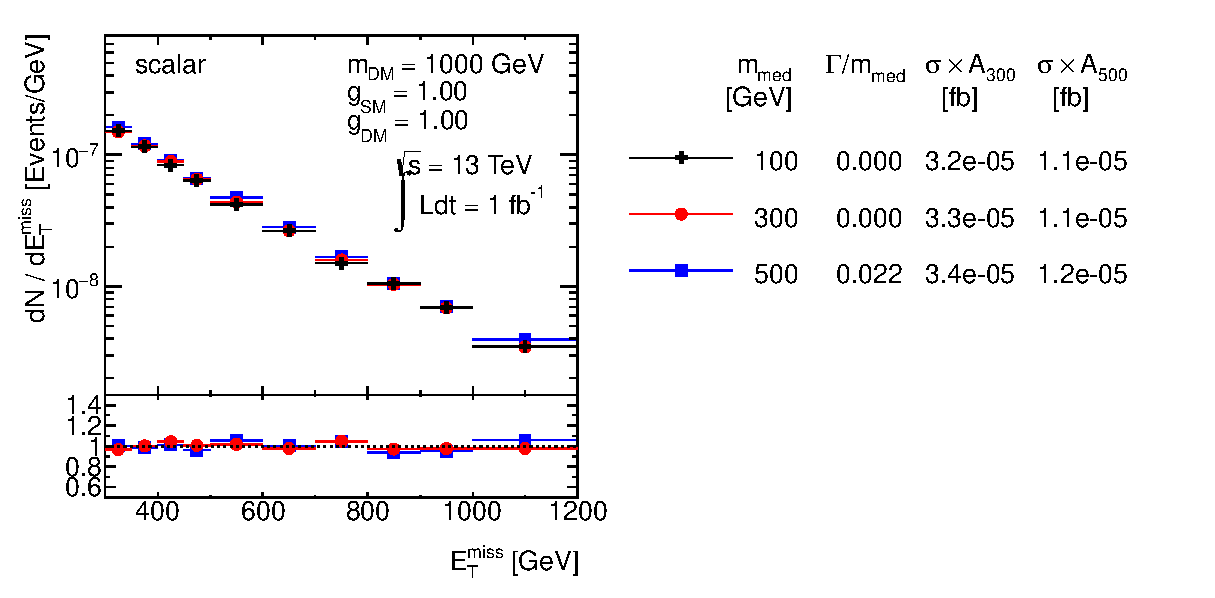
\includegraphics[width=0.9\textwidth]{figures/monojet/scan_mMed_S_1000.eps}
\caption{Scan over mediator mass. The $\MET$ distribution is compared for the scalar mediator models using the parameters as indicated. Ratios of the normalized distributions with respect to the first one are shown. $A_{300}$ and $A_{500}$ in the table denote the acceptance of the $\MET>300$~\gev and $\MET>500$~\gev cut, respectively.}
\label{fig:monojet_scan_S_mMed1000}
\end{figure}


The optimized parameter grid in the $\mMed$--$\mDM$ plane for scalar and pseudo-scalar mediators is motivated by similar arguments as in the previous section. Therefore, a similar pattern is followed here, taking again $\gq=\gDM=1$. Only the sensitivity to the highest mediator masses has to be re-evaluated.
The generator level cross section times the acceptance at $\MET>500$~\gev for the model with couplings $\gq=\gDM=1$, light Dark Matter of \mDM=10~\gev and
a \mMed=500~\gev scalar mediator is at the order of 10\,fb, i.e. just at the edge of the early Run-2 sensitivity. Increasing the mediator mass to 1~\tev pushes the product $\sigma\times A$ down to approximately 0.1\,fb, below the LHC sensitivity. Therefore, we choose to remove the 2~\tev mediator mass from the grid and present the final grid with 32
%26 
mass points only, as shown in Tab.\,\ref{tab:mDMmMedScan_SP}.
One point at very high mediator mass (5~\tev) is added for each of the DM masses scanned, to aid the reinterpretation of results in terms of contact interaction operators (EFTs). 

\begin{table}[!h]
\centering
\begin{tabular}{| l |r r r r r r r r r|}
\hline
\multicolumn{1}{|c|}{\mDM (\gev)} & \multicolumn{9}{c|}{\mmed (\gev)} \\
\hline
 1             &         10  & 20 & 50 & 100 & 200 & 300 & 500 &         1000  &         5000  \\
 10   	       &         10  & 15 & 50 & 100 &     &     &     &               &         5000  \\
 50            &         10  &    & 50 &  95 & 200 & 300 &     &               &         5000  \\
 150           &         10  &    &    &     & 200 & 295 & 500 &               &         5000  \\
 500           &         10  &    &    &     &     &     & 500 &          995  &         5000  \\
 1000          &         10  &    &    &     &     &     &     &         1000  &         5000  \\
\hline
\end{tabular}

\caption{Simplified model benchmarks for $s-$channel simplified models (spin-0 mediators 
decaying to Dirac DM fermions in the scalar and pseudoscalar case, taking the minimum width for \gq = \gDM = 1)}.
% Points in \textbf{bold} are only generated for the vector/axial vector cases, while points in 
% \textit{italics} are generated for the monojet analysis 
% but not for the search including heavy quarks. This table corresponds to 29 points for monojet vector/axial vector models,
% 26 points for monojet scalar/pseudoscalar models and 24 points for $t \bar{t}$+\MET scalar/pseudoscalar models.}

\label{tab:mDMmMedScan_SP}
% \end{sidewaystable}
\end{table}

% \begin{figure}
% \centering
% 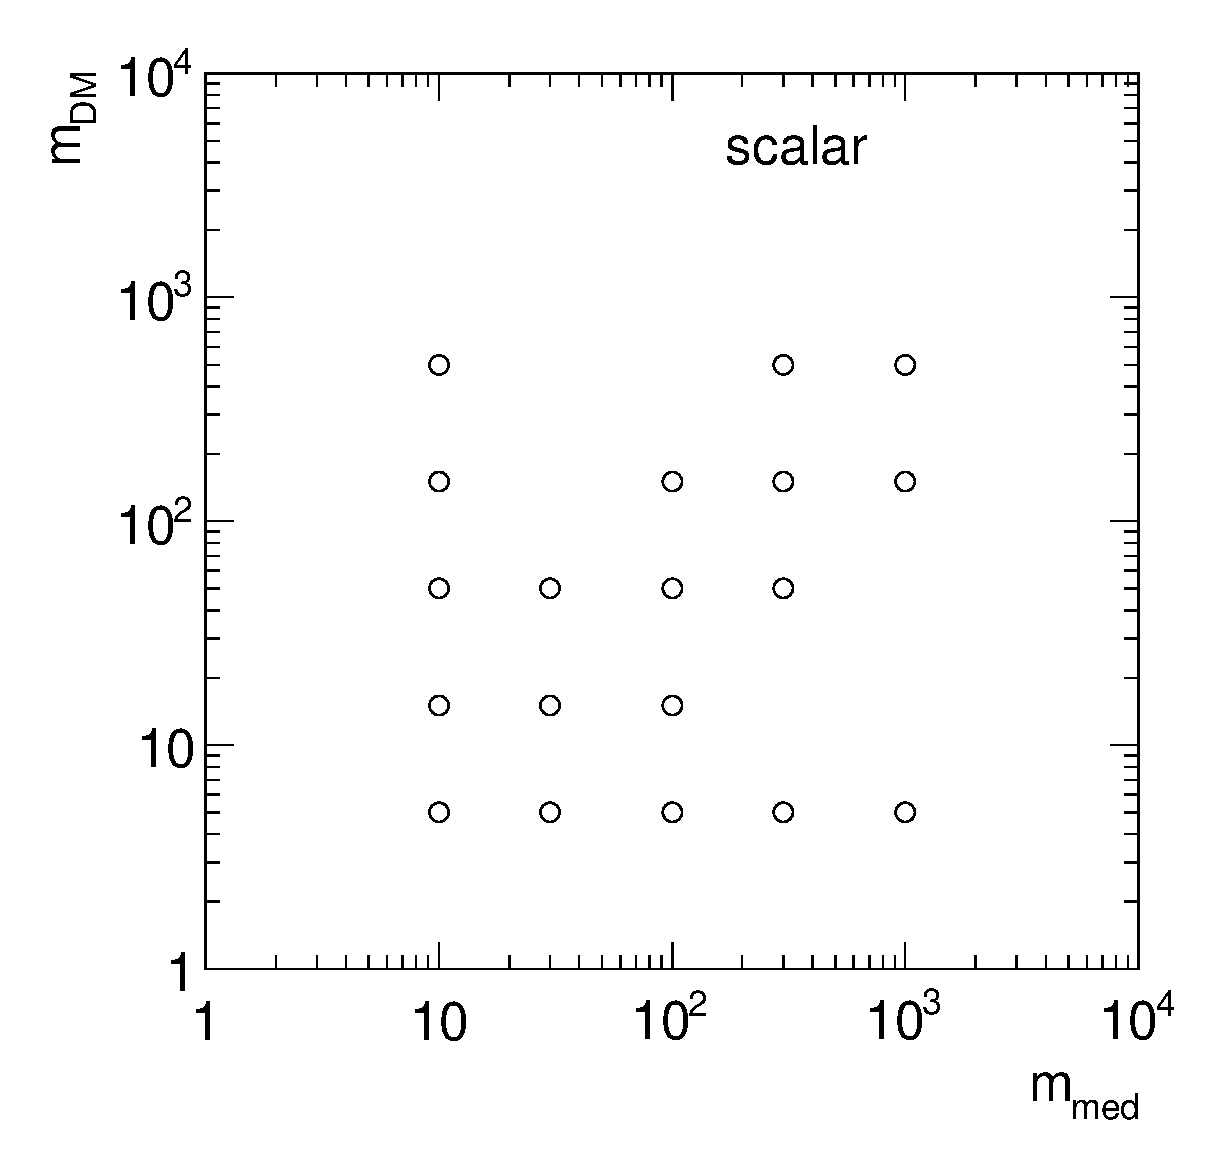
\includegraphics[width=0.45\textwidth]{figures/monojet/grid_S.eps}
% 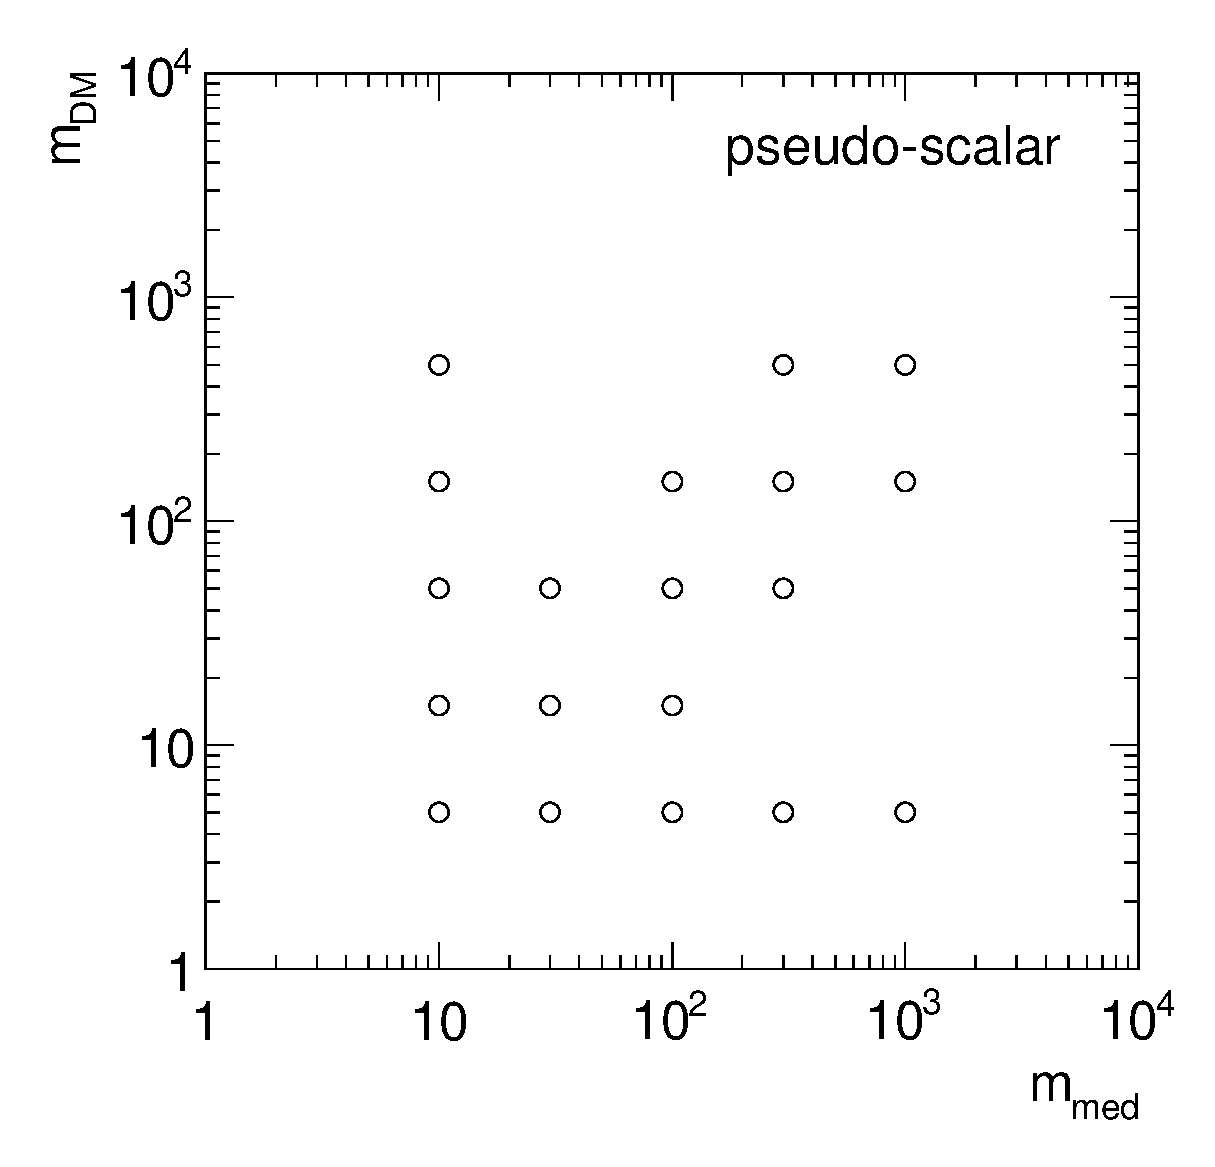
\includegraphics[width=0.45\textwidth]{figures/monojet/grid_P.eps}
% \caption{Proposed parameter grid for scalar and pseudo-scalar mediator in the $\mMed$--$\mDM$ plane.}
% \label{fig:monojet_grid_S}
% \end{figure}

The proposal for the scan in the $\gq$--$\gDM$ plane is described in the following section.




\section{Presentation of results for reinterpretation}
\label{sec:monojet_scaling}

The aim of the parameter grid optimization is to
reduce the parameter space for simulation
using neighboring grid points to populate the missing parts.
Two ways of doing this are:
\begin{itemize}
\item Interpolation is used in-between the grid points that are close enough such that finer granularity is not needed for the presentation purposes, or between the points where smooth or no changes of the results are expected. The latter argument is exactly the one that motivates the reduction of the grid points in the $\mMed$--$\mDM$ plane.\\
\item Recalculation of the results can be used when the dependencies with respect to the neighboring grid points are known.\\
\end{itemize}

The results of the scan over the couplings presented in the previous sections indicate there are no changes in kinematic distributions for different choices of the coupling strengths. This means that the acceptance remains the same in the whole $\gq$--$\gDM$ plane and it is sufficient to perform the detector simulation only for one single choice of $\gq, \gDM$. The resulting truth-level selection acceptance and the detector reconstruction efficiency can then be applied to all remaining grid points in the $\gq$--$\gDM$ plane where only the generator-level cross section needs to be known. This significantly reduces the computing time as the detector response is by far the most expensive part of the Monte Carlo sample production.
However,
the number of generated samples can be reduced even further
if a parameterization of the cross section dependence from one grid point to another exists.

Let us now elaborate on a cross section scaling procedure.~\Todo{This procedure needs a clarification: this can work only for fixed masses}
%TODO say something about the fact that this can work only for fixed masses
The propagator on the \schannel exchange is written in a Breit-Wigner form as $\frac{1}{q^2-\mMed^2 + i\mMed\Gamma}$, where $q$ is the momentum transfer calculated from the two partons entering the hard process after the initial state radiation, which is equivalent to the invariant mass of the Dark Matter pair. %The relative size of the center-of-mass energy defined by the two partons entering the hard process and the mediator mass allows to classify the production in the following way:
The size of the momentum transfer with respect to the mediator mass allows to classify the production in the following way:
\begin{itemize}
\item off-shell production when $q^2 \gg \mMed$ leading to suppressed cross sections,
\item on-shell production when $q^2 \sim \mMed$ leading to enhanced cross sections,
\item effective field theory (EFT) limit when $q^2 \ll \mMed$.
\end{itemize}
All three categories can be distinguished in Fig.\,\ref{fig:monojet_MstarMmed} showing the upper limit on the interaction scale $M^{*} \equiv \mMed/\sqrt{\gq\gDM}$ for vector mediator. 
In the case of the off-shell production and the EFT limit, the first and second term in the propagator dominate, respectively, which reduces the dependence on the mediator width. Therefore, in these cases one can approximate the cross section as
\begin{equation}
\sigma \propto \gq^2\gDM^2.
\end{equation}
The on-shell production regime is the most interesting one as it gives the best chances for a discovery at the LHC given the cross section enhancement. The propagator term with the width cannot be neglected in this case and, in the narrow width approximation which requires $\Gamma \ll \mMed$ (this is not necessarily the case in the benchmarks considered in the scans), one can integrate
\begin{equation}
\int \frac{ds}{(s-\mMed^2)^2 + \mMed^2\Gamma^2} = \frac{\pi}{\mMed\Gamma}
\label{eq:monojet_int}
\end{equation}
which further implies the cross section scaling
\begin{equation}
\sigma \propto \frac{\gq^2\gDM^2}{\Gamma}.
\label{eq:monojet_scaling}
\end{equation}
The narrow with approximation is important here as it ensures an integration over parton distribution functions (PDFs) can be neglected. In other words, it is assumed the integrand in Eq.\,\ref{eq:monojet_int} is non-zero only for a small region of $s$, such that the PDFs can be taken to be constant in this range.
Since $\Gamma \sim \gq^2+\gDM^2$, one can simplify this rule in the extreme cases as follows
\begin{eqnarray}
\sigma &\propto& \frac{\gq^2\gDM^2}{\gq^2+\gDM^2} \xrightarrow{\gq \ll \gDM} \gq^2 \label{eq:monojet_gSM} \\
\sigma &\propto& \frac{\gq^2\gDM^2}{\gq^2+\gDM^2} \xrightarrow{\gq \gg \gDM} \gDM^2 \label{eq:monojet_gDM} \;.
\end{eqnarray}
%However, it is important to keep in mind that there is no simple scaling rule for how the cross section changes with the Dark Matter mass, mediator mass and the mediator width because PDFs matter in such cases as well.
%The only case where there is a simple scaling with mass is if one mass is much smaller than the other mass, in which case the cross section becomes independent of the smaller mass.
However, it is important to keep in mind that this formula omits color and multiplicity factors as well as possible Yukawa suppression, and there is no simple scaling rule for how the cross section changes with the Dark Matter mass and the mediator mass, or for mediators with a large width, because PDFs matter in such cases as well.
Therefore, the scaling procedure outlined above is expected to work only for fixed masses and fixed mediator width, assuming the narrow width approximation applies.


\begin{figure}
\centering
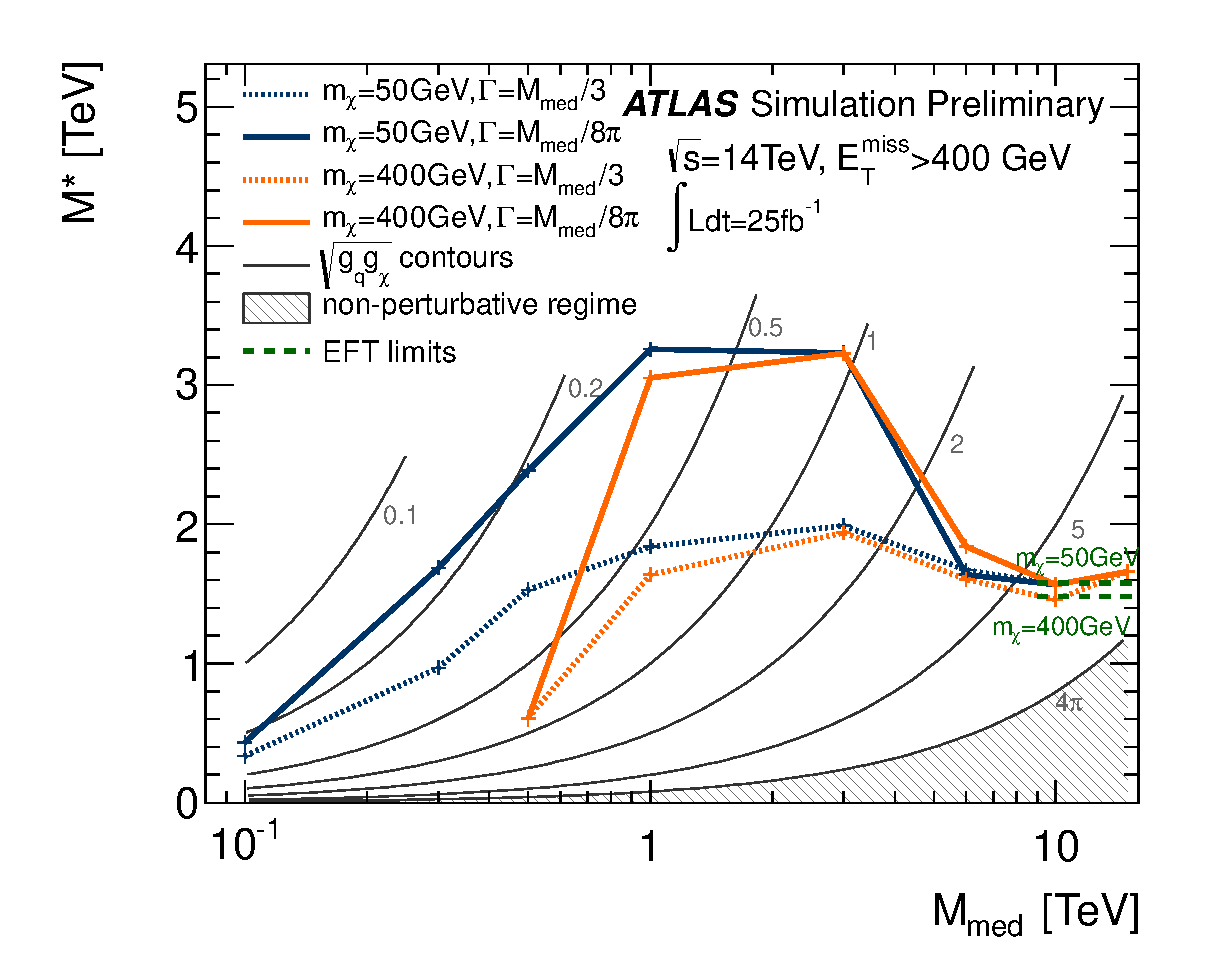
\includegraphics[width=0.9\textwidth]{figures/monojet/lambda_14TeV_SR1.eps}
\caption{Comparison of the 95\% CL lower limits on the scale of the interaction of a \Zprime-like simplified model at 14~\tev, in terms of the mediator mass. Corresponding limits from EFT models are shown on the same plot as green dashed lines to show equivalence between the two models for high mediator masses.
Taken from Ref.\,\cite{ATL-PHYS-PUB-2014-007}.}
\label{fig:monojet_MstarMmed}
\end{figure}


\Todo{Indicate mMed=GammaMin in the plots (gDM = 6, gSM = 1.5 for $V$ and gSM = gDM = 5 for $S$)}

Figures\,\ref{fig:monojet_width100} and \ref{fig:monojet_width1000} show the minimal width in the $\gq$--$\gDM$ plane for all vector, axial-vector, scalar and pseudo-scalar mediators for $\mMed=100$~\gev and 1000~\gev, respectively, taking $\mDM=10$~\gev. The individual colors indicate the lines of constant width along which the cross section scaling works. For vector and axial-vector mediators, the minimal width is predominantly defined by $\gq$ due to the number of quark flavors and the color factor. %In this case, the scaling follows from Eq.\,\ref{eq:monojet_gDM}.
On the contrary, both the Standard Model and Dark Matter partial width have comparable contributions in case of scalar and pseudo-scalar mediators if the top quark channel is open ($\mMed>2m_t$). However, mostly $\gDM$ defines the minimal width for $\mMed<2m_t$ due to the Yukawa-suppressed light quark couplings.



\begin{figure}
\centering
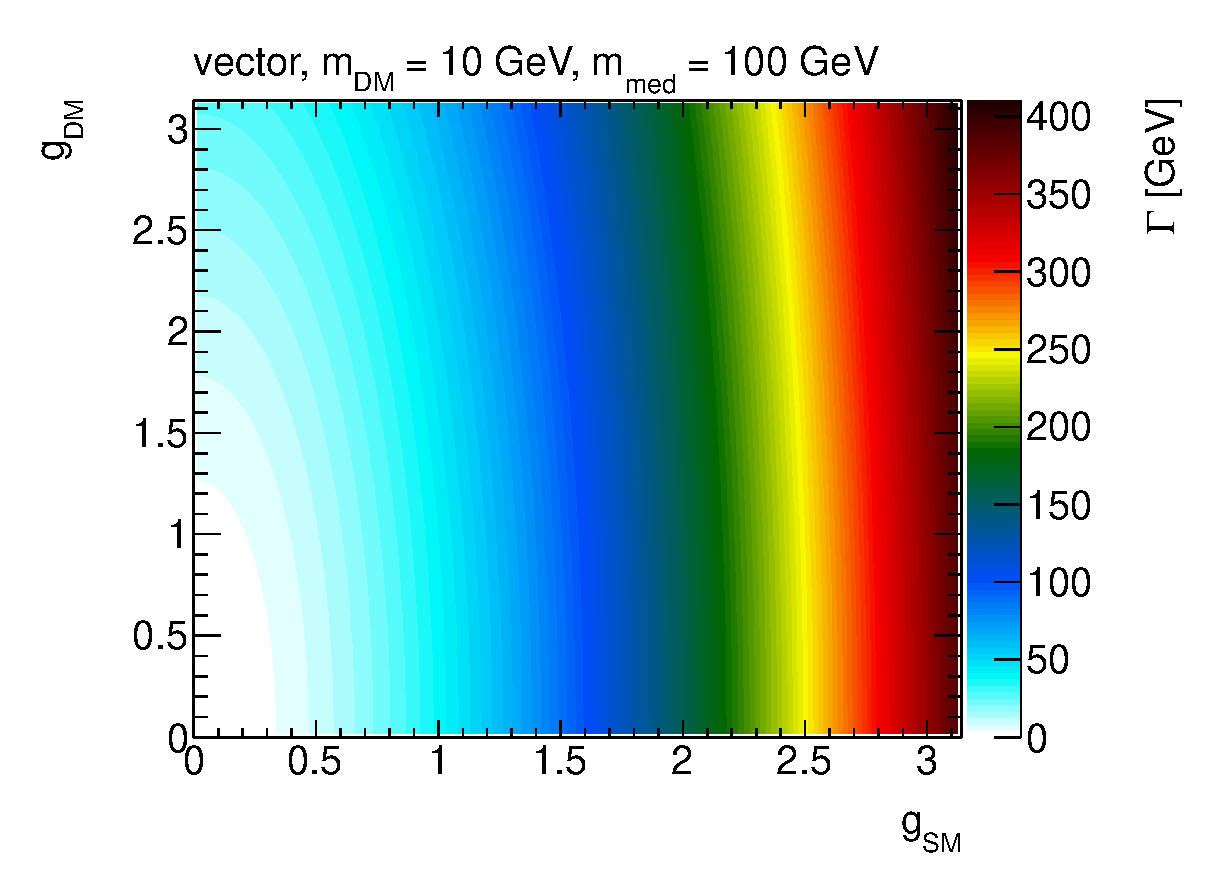
\includegraphics[width=0.45\textwidth]{figures/monojet/constantwidth_V_gg100.eps}
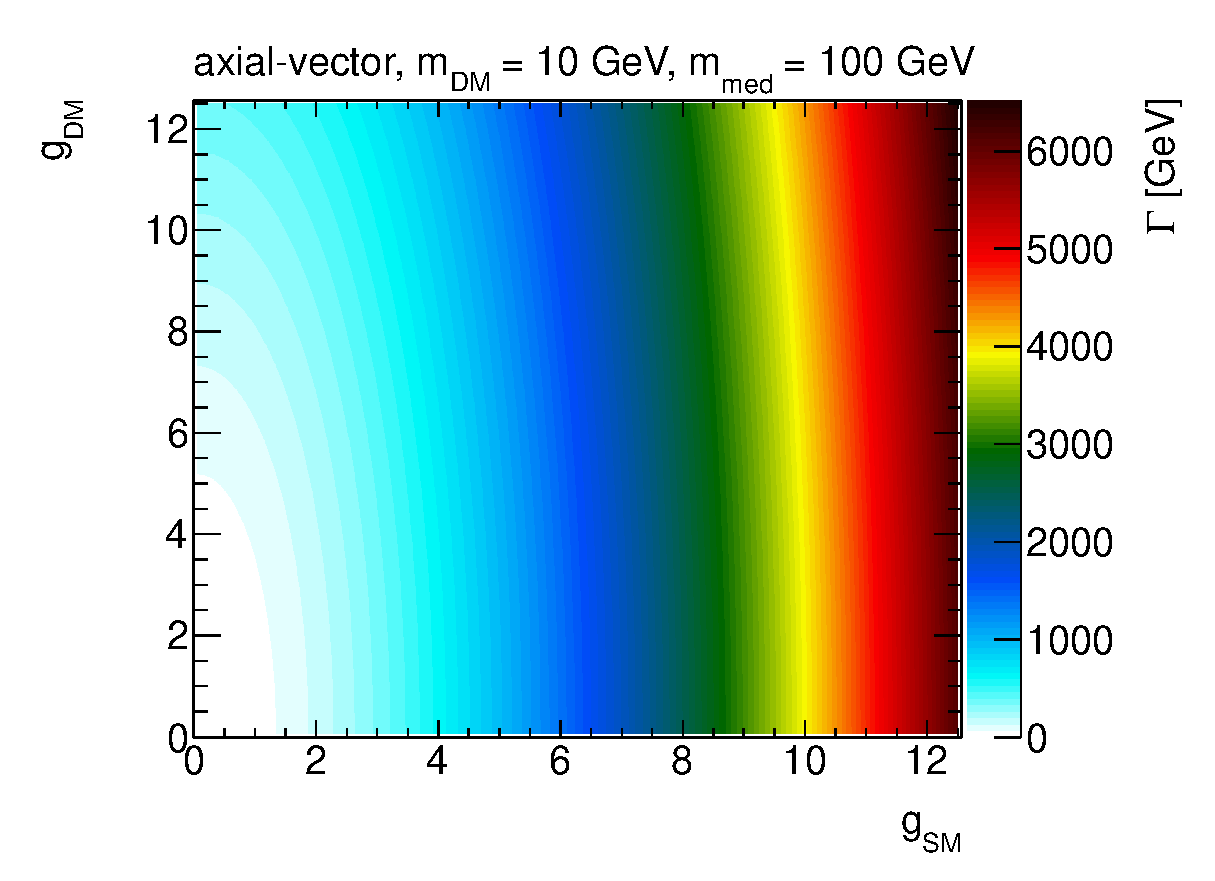
\includegraphics[width=0.45\textwidth]{figures/monojet/constantwidth_A_gg100.eps}\\
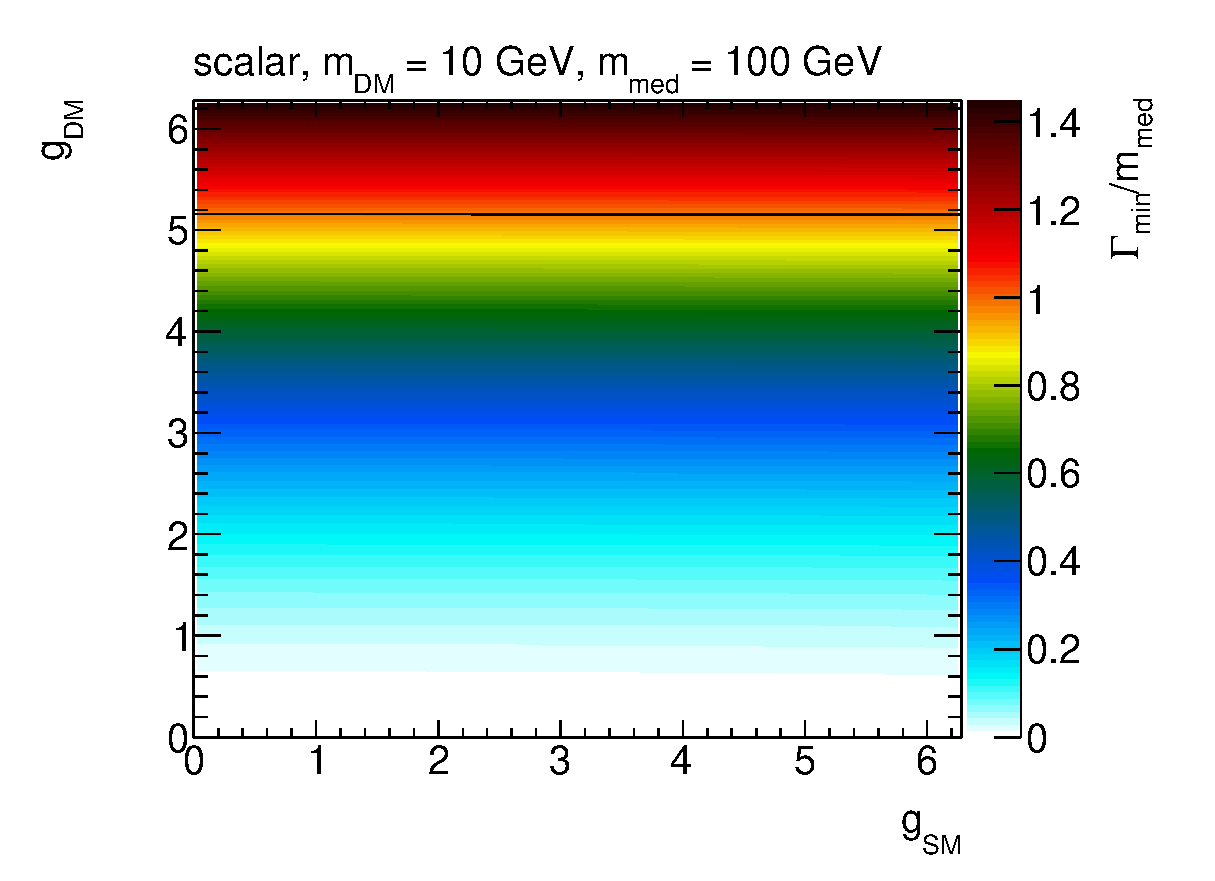
\includegraphics[width=0.45\textwidth]{figures/monojet/constantwidth_S_gg100.eps}
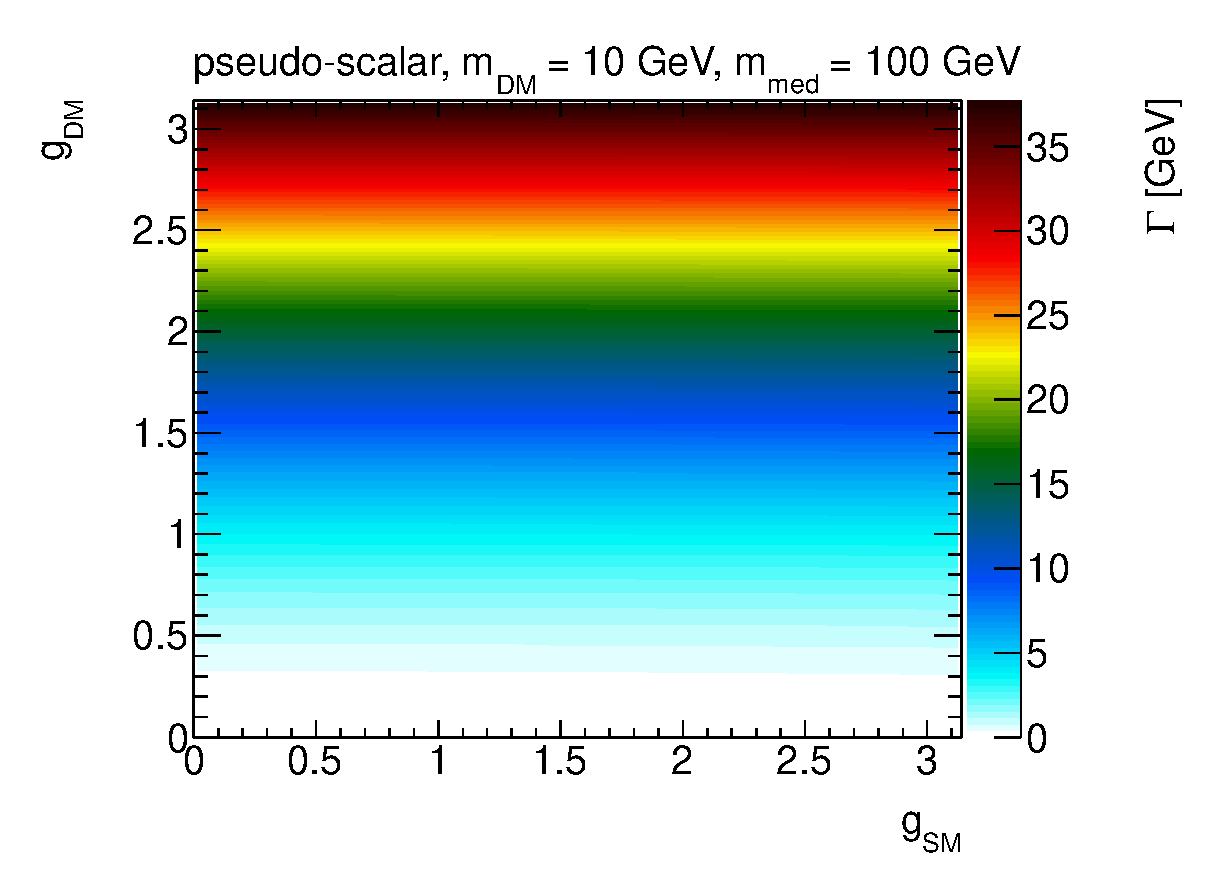
\includegraphics[width=0.45\textwidth]{figures/monojet/constantwidth_P_gg100.eps}
\caption{Minimal width for vector, axial-vector, scalar and pseudo-scalar mediators as a function of the individual couplings $\gq$ and $\gDM$, assuming $\mMed=100$~\gev and $\mDM=10$~\gev.
The limiting case $\Gamma_{\rm{min}}=\mMed$ is indicated by the black line.} 
\label{fig:monojet_width100}
\end{figure}

\begin{figure}
\centering
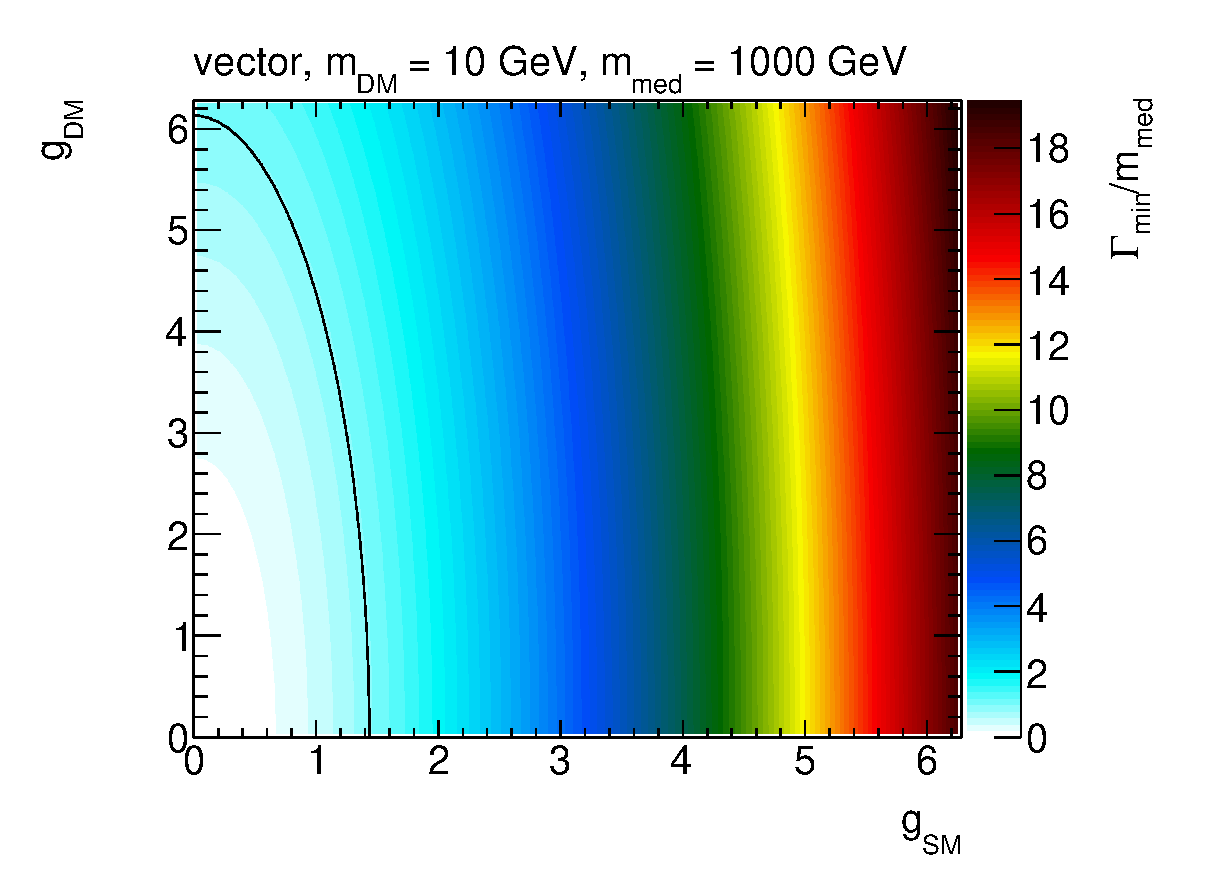
\includegraphics[width=0.45\textwidth]{figures/monojet/constantwidth_V_gg1000.eps}
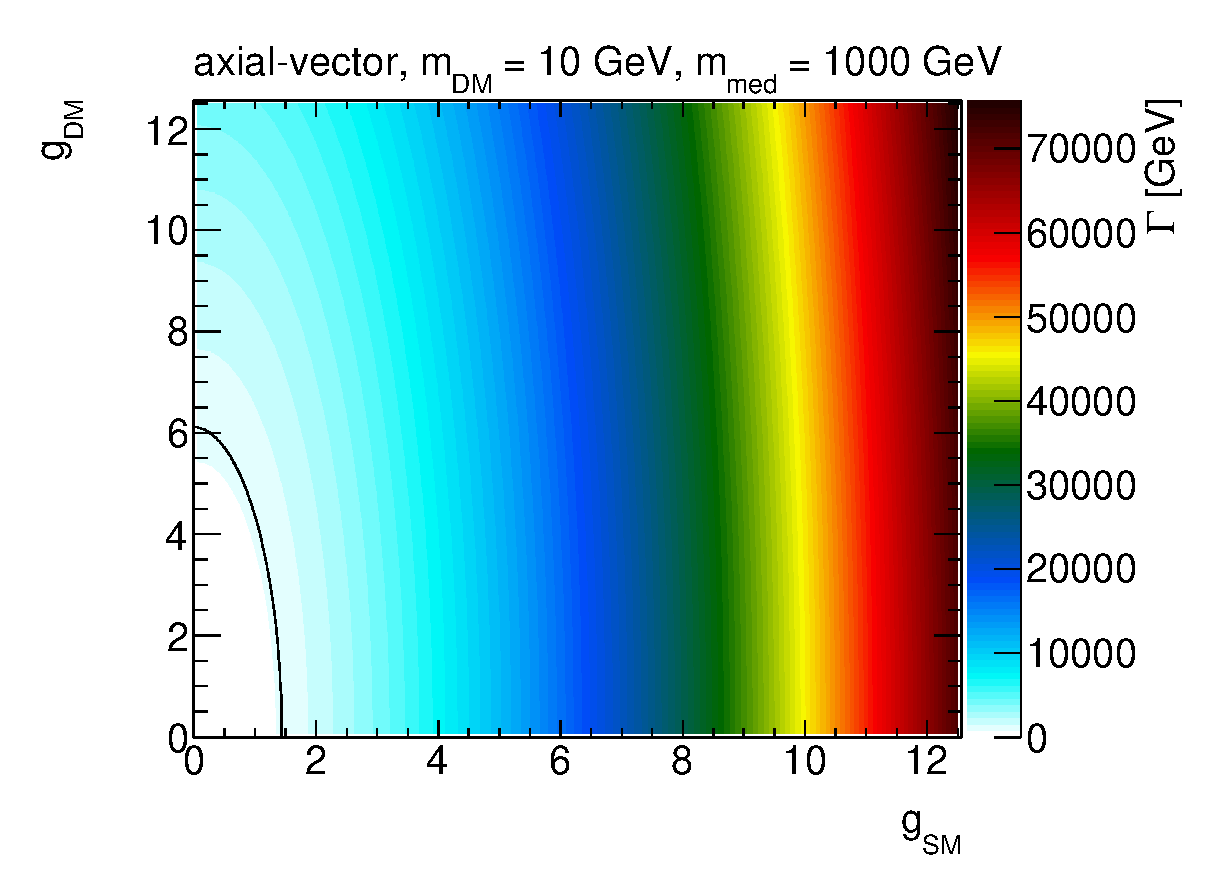
\includegraphics[width=0.45\textwidth]{figures/monojet/constantwidth_A_gg1000.eps}\\
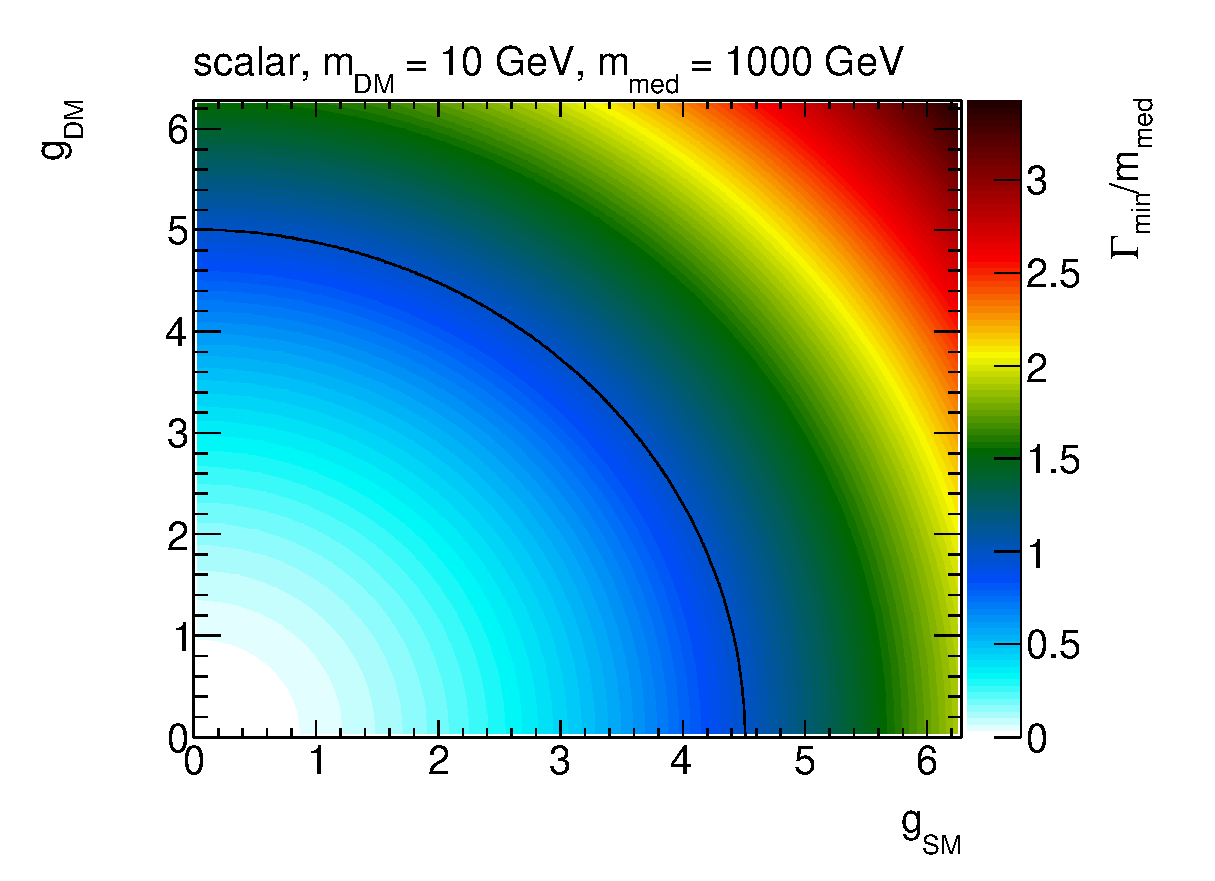
\includegraphics[width=0.45\textwidth]{figures/monojet/constantwidth_S_gg1000.eps}
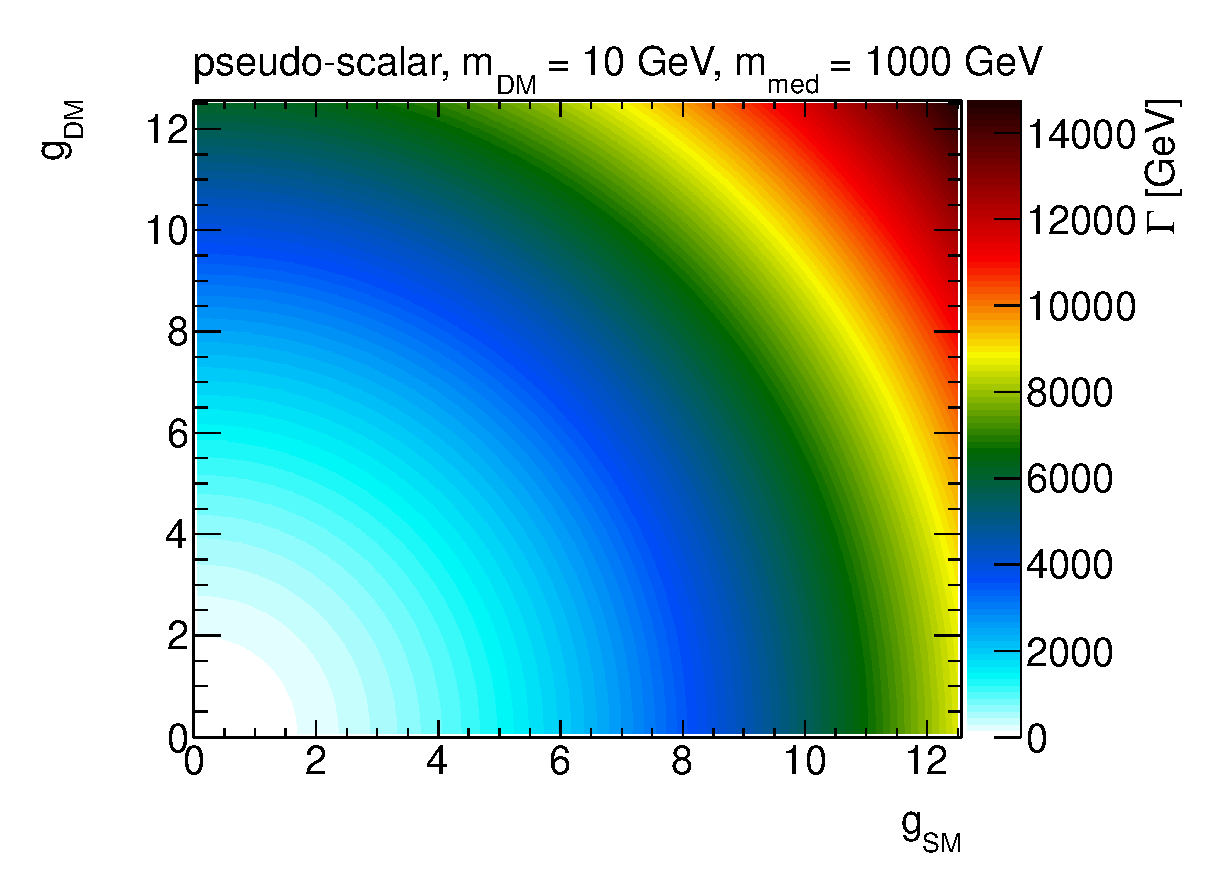
\includegraphics[width=0.45\textwidth]{figures/monojet/constantwidth_P_gg1000.eps}
\caption{Minimal width for vector, axial-vector, scalar and pseudo-scalar mediators as a function of the individual couplings $\gq$ and $\gDM$, assuming $\mMed=1$~\tev and $\mDM=10$~\gev.
The limiting case $\Gamma_{\rm{min}}=\mMed$ is indicated by the black line.} 
\label{fig:monojet_width1000}
\end{figure}


The performance of the cross section scaling is demonstrated in Fig.\,\ref{fig:monojet_scaling} %where two mass points $\mMed=100$~\gev and 1~\tev are chosen with $\mDM=10$~\gev
where two mass points $\mMed=100$~\gev and 1~\tev with $\mDM=10$~\gev are chosen
and rescaled from the starting point $\gq=\gDM=1$ according to Eq.\,\ref{eq:monojet_scaling} to populate the whole $\gq$--$\gDM$ plane. This means the width is not kept constant in this test and this is done in purpose in order to point out deviations from the scaling when the width is altered. For each mass point, the rescaled cross section is compared to the generator cross section and the ratio of the two is plotted.
For the given choice of the mass points, the scaling seems to work approximately with the precision of $\sim20\%$ in the region where $\Gamma_{\rm{min}}<\mMed$.
Constant colors indicate the lines along which the cross section scaling works precisely and there is a remarkable resemblance of the patterns shown in the plots of the mediator width. To prove the scaling along the lines of constant width works, one such line is chosen in Fig.\,\ref{fig:monojet_scaling_constwidth} for a scalar mediator, defined by $\mMed=300$~\gev, $\mDM=100$~\gev, $\gq=\gDM=1$, and the rescaled and generated cross sections are found to agree within 3\%.


\begin{figure}
\centering
%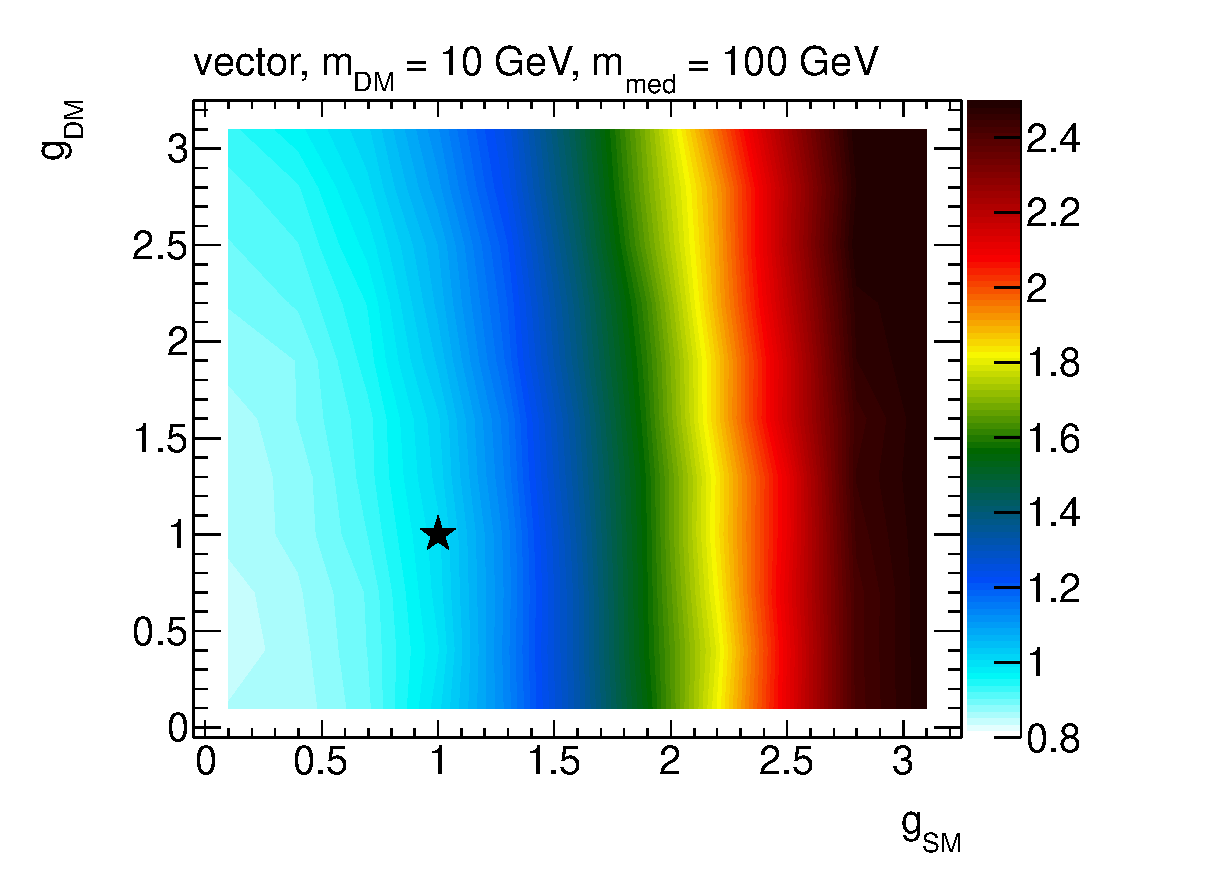
\includegraphics[width=0.45\textwidth]{figures/monojet/scaling_V_10_100.eps}
%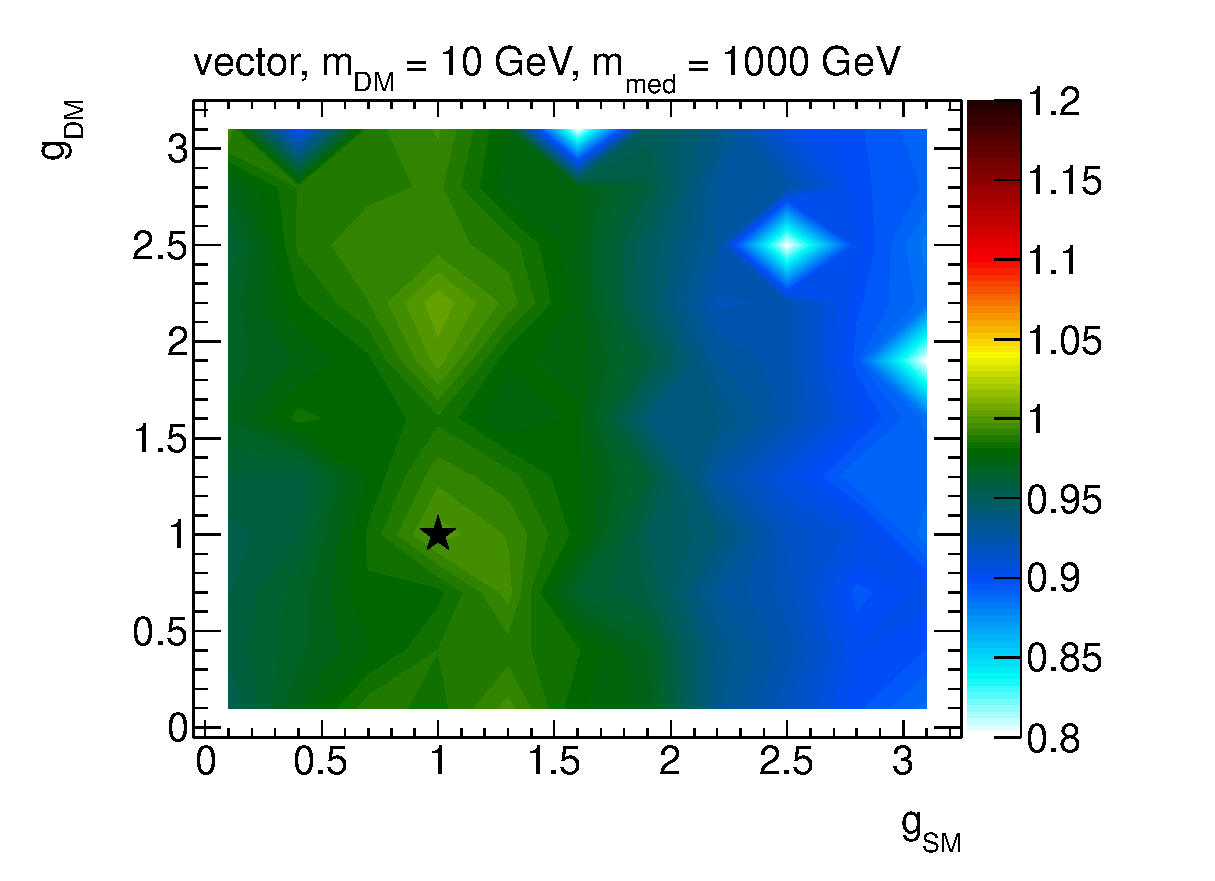
\includegraphics[width=0.45\textwidth]{figures/monojet/scaling_V_10_1000.eps}\\
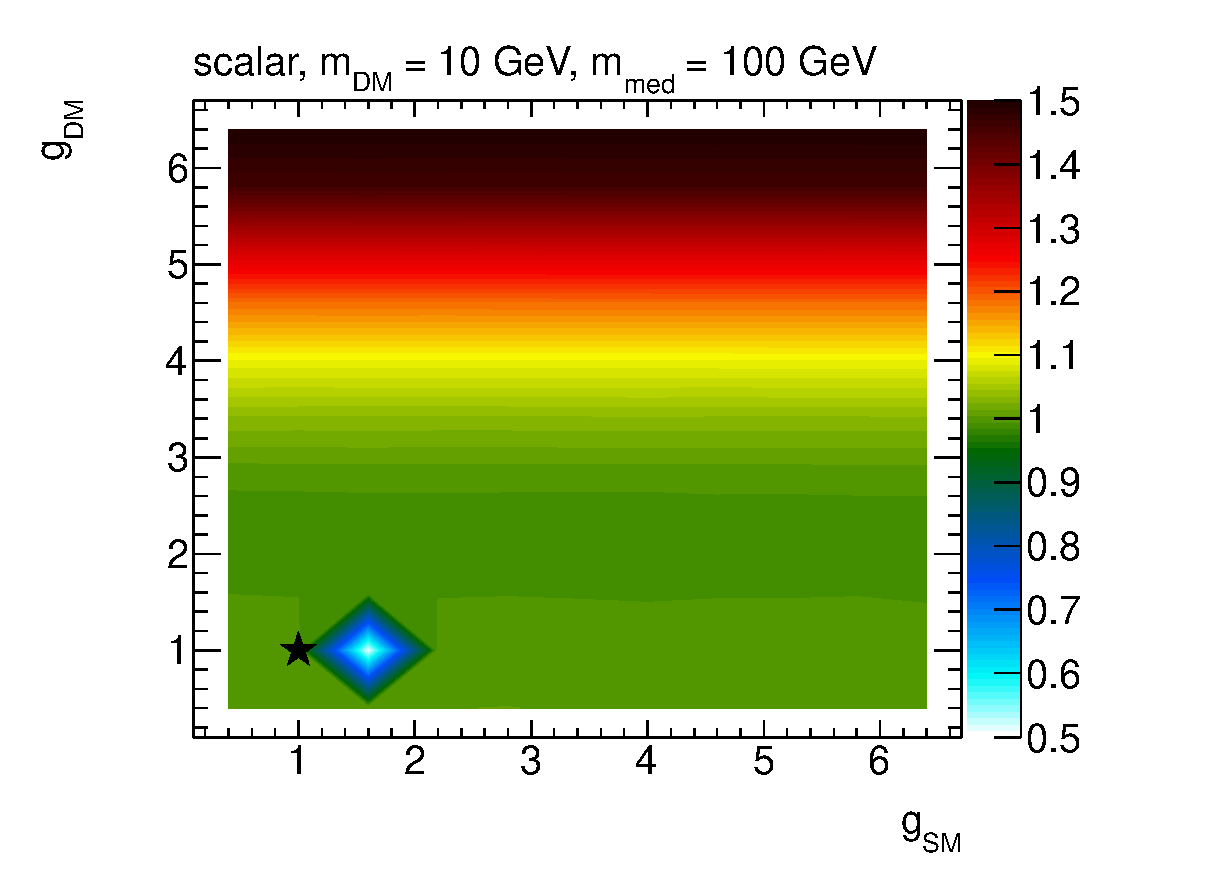
\includegraphics[width=0.45\textwidth]{figures/monojet/scaling_S_10_100.eps}
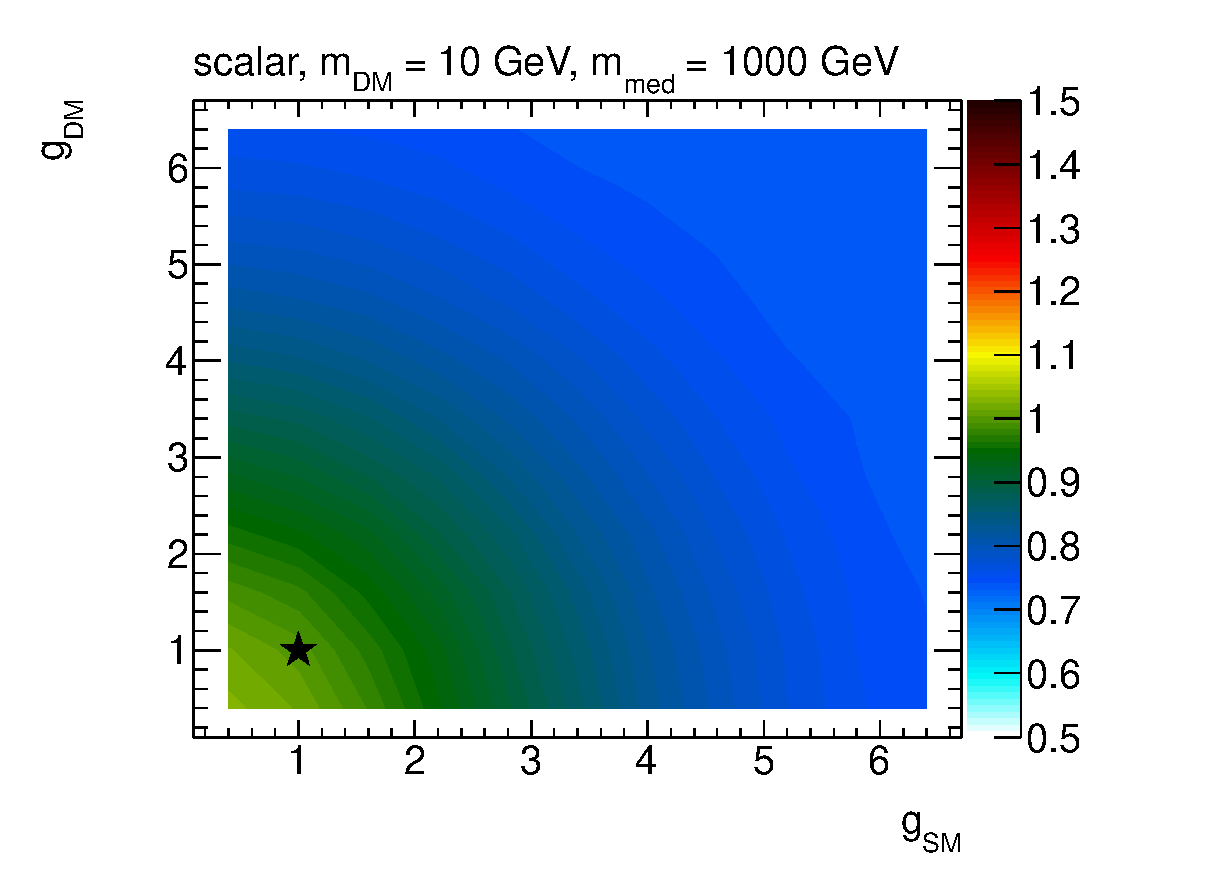
\includegraphics[width=0.45\textwidth]{figures/monojet/scaling_S_10_1000.eps}\\
\caption{Ratio of the rescaled and generated cross sections in the $\gq$--$\gDM$ plane. The point at $\gq=\gDM=1$, taken as a reference for the rescaling, is denoted by a star symbol.
Scalar model with $\mMed=100$~\gev (left) and 1~\tev (right) is plotted for $\mDM=10$~\gev.
The limiting case $\Gamma_{\rm{min}}=\mMed$ is shown as a black line.}
%Vector (scalar) mediator is shown at the top (bottom), the left (right) column corresponds to $\mMed=100$~\gev ($\mMed=1$~\tev). Dark Matter mass of 10~\gev is considered.}
\label{fig:monojet_scaling}
\end{figure}

%The plots are produced with M_S = 300~\gev, m_chi = 100~\gev, \gSM = \gDM =4
\begin{figure}
\centering
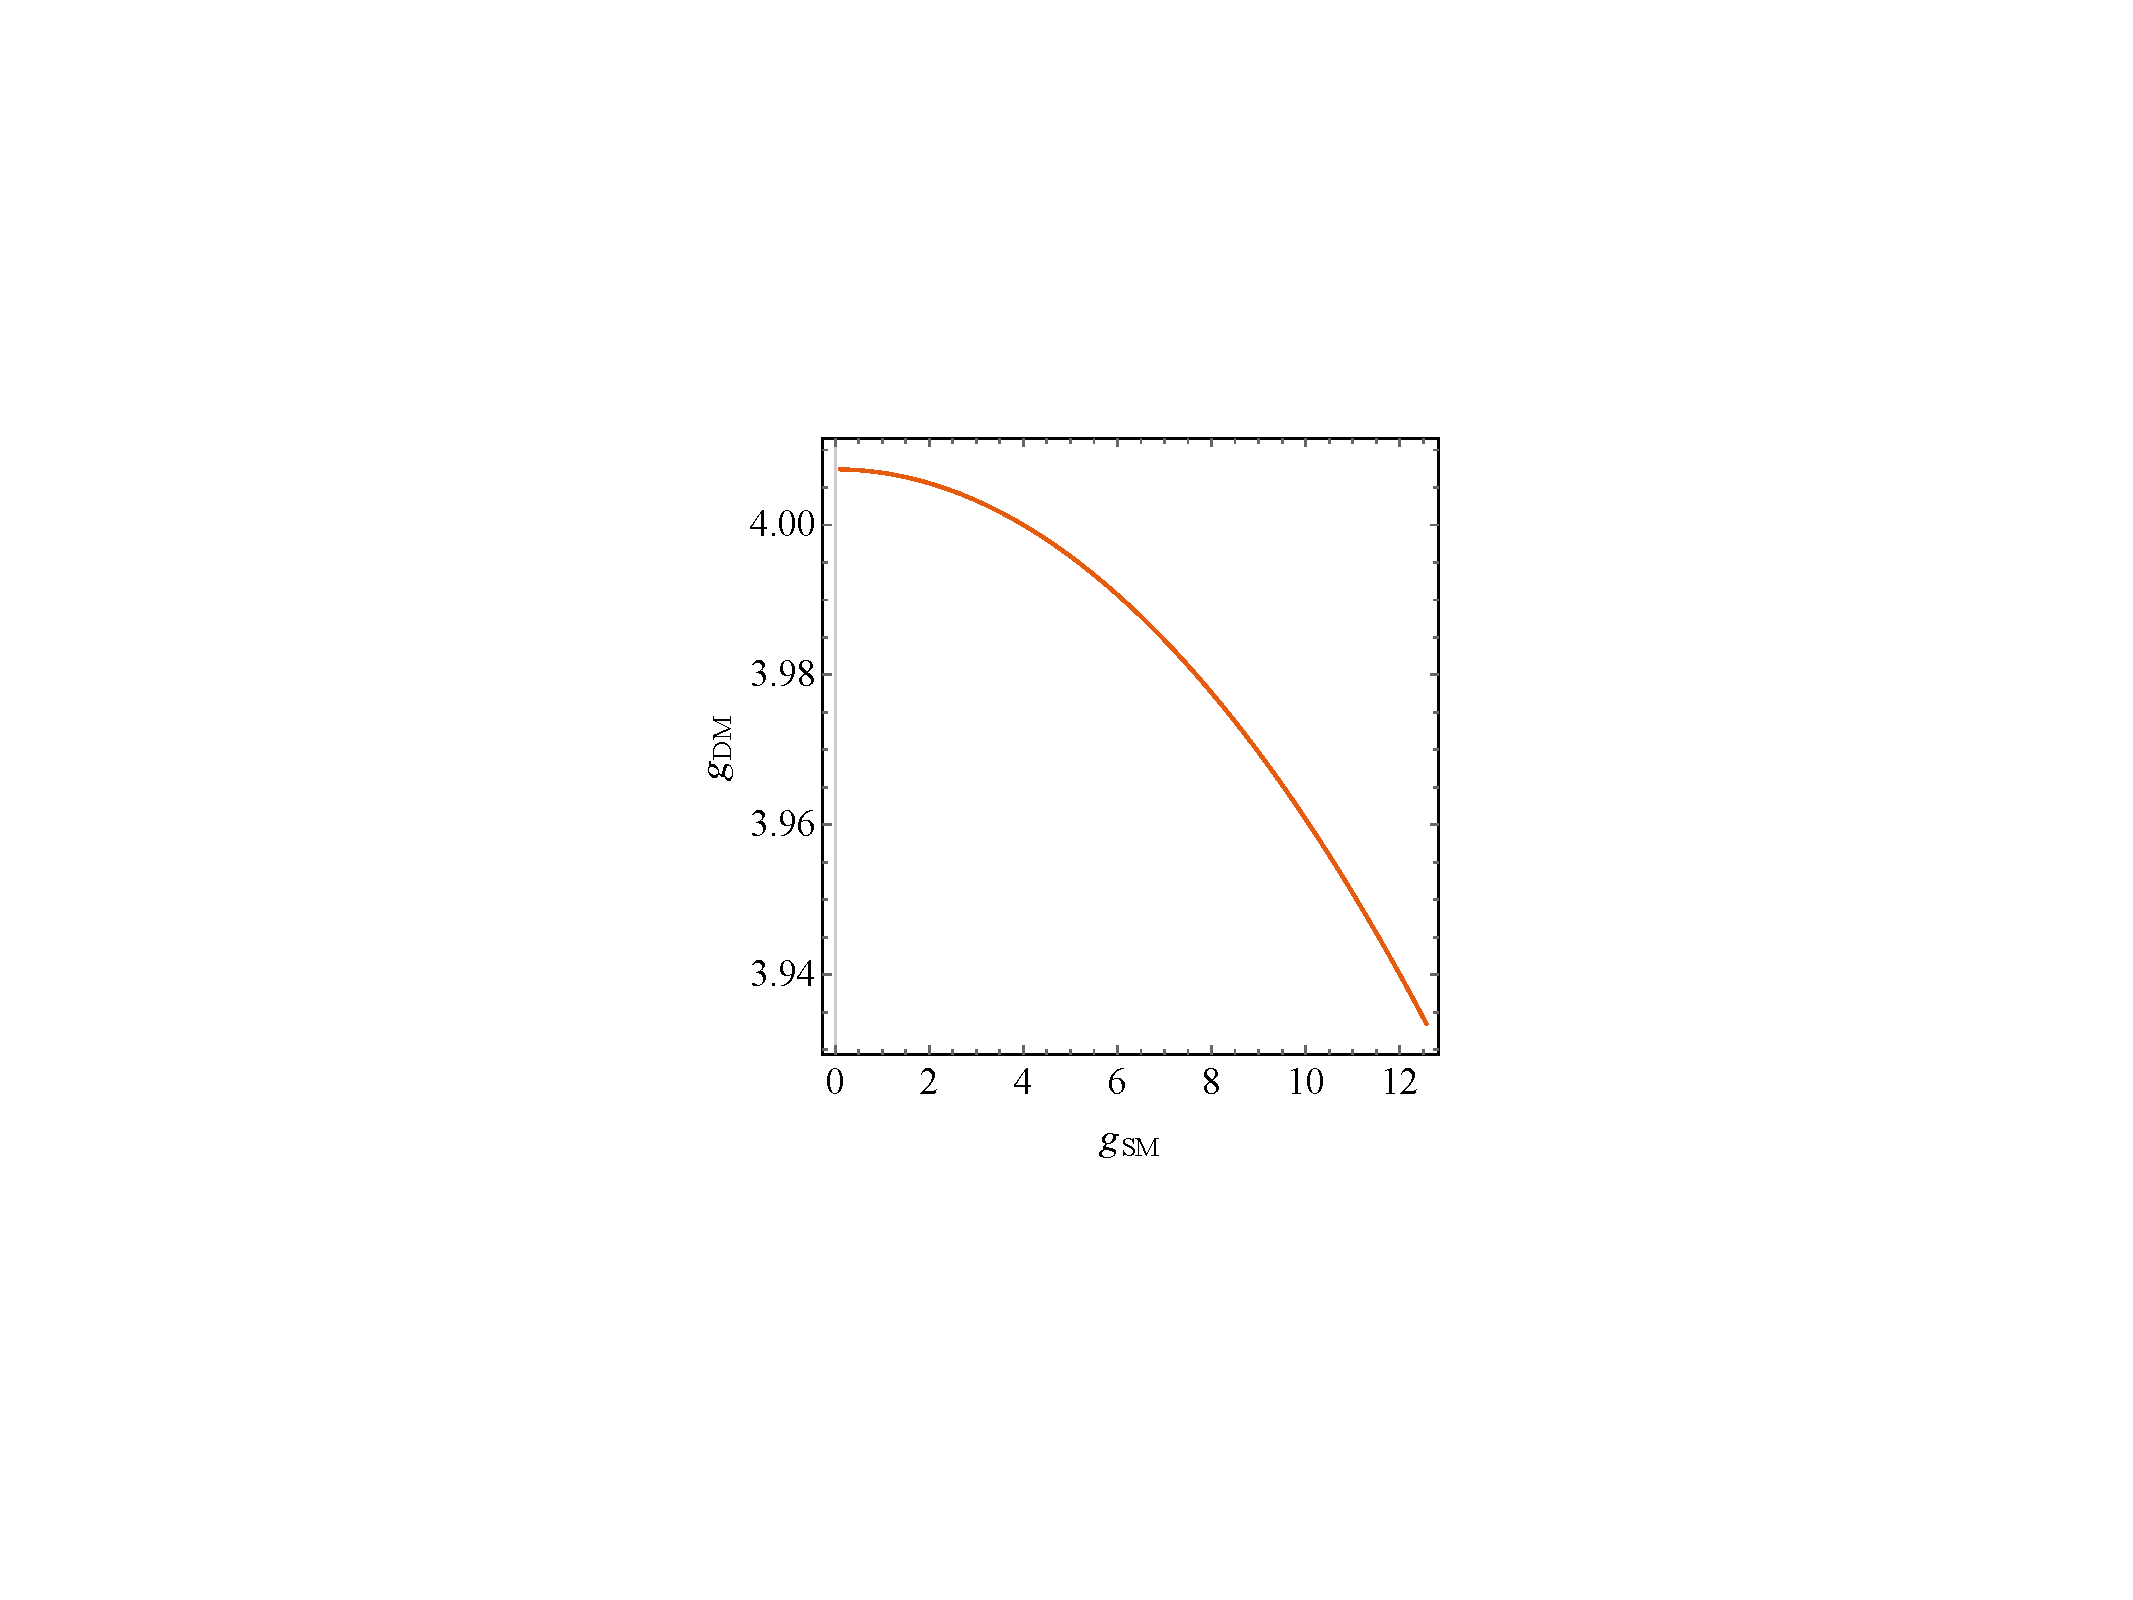
\includegraphics[page=1, trim=310 200 310 200, clip, width=0.3\textwidth]{figures/monojet/rescalingexercise.pdf}
\includegraphics[page=2, trim=305 195 305 195, clip, width=0.3\textwidth]{figures/monojet/rescalingexercise.pdf}
\includegraphics[page=3, trim=300 190 300 190, clip, width=0.3\textwidth]{figures/monojet/rescalingexercise.pdf}
\caption{Scaling along the lines of constant width. The line of constant width for $\mMed=300$~\gev and $\mDM=100$~\gev, intercepting $\gq=\gDM=4$ is shown on left. The generated and rescaled cross sections are compared in the middle, the corresponding ratio is shown on right.}
%TODO ask Uli for the color code
\label{fig:monojet_scaling_constwidth}
\end{figure}


\paragraph{Proposed parameter grid for cross-section scaling}

We propose to present the results in the $\gq$--$\gDM$ plane using the following prescription:
\begin{itemize}
\item Since the shapes of kinematic quantities do not change for different couplings, use the acceptance and efficiency for the available $\mDM=50$~\gev, $\mMed=300$~\gev, $\gq=\gDM=1$ grid point from the $\mMed$--$\mDM$ plane for the scalar and pseudo-scalar mediator. In case of the vector and axial-vector mediator, use the grid point $\mDM=50$~\gev, $\mMed=1$~\tev, $\gq=\gDM=1$.
\item Generate additional samples in order to get generator cross sections only. For scalar and pseudo-scalar mediator, choose $\mDM=50$~\gev, $\mMed=300$~\gev with the following values for $\gq=\gDM$: 0.1, 1, 2, 3. For vector and axial vector mediator, choose $\mDM=50$~\gev, $\mMed=1$~\tev with the following values for $\gq=\gDM$: 0.1, 0.25, 0.5, 0.75, 1.25, 1.5. The upper values are defined by the minimal width reaching the mediator mass. \Todo{Waiting for scalar mediator calculation of perturbativity limit from J. Alcaraz.).}
\item Rescale the generator cross sections for on-shell resonance production along the lines of constant width in order to populate the whole $\gq$--$\gDM$ plane.
\end{itemize}

%choose mDM=50, mMed=300, gSM=0.1, gDM={0.1, 1, 2, 3, 4, 5, 6} for S (mMed=GammaMin is reached around 5)
%choose mDM=50, mMed=300, gDM=0.1, gSM={0.1, 0.4, 0.7, 1, 1.3, 1.6, 1.9} for V (mMed=GammaMin is reached around 1.6)
%choose mDM=50, mMed=1000, gDM=0.1, gSM={0.1, 0.4, 0.7, 1, 1.3, 1.6, 1.9} for V (mMed=GammaMin is reached around 1.5)

%choose mDM=50, mMed=300, gSM=gDM={0.1, 1, 2, 3, 4, 5, 6} for S (mMed=GammaMin is reached around 5)
%choose mDM=50, mMed=300, gDM=gSM={0.1, 0.25, 0.5, 0.75, 1, 1.25, 1.5} for V (mMed=GammaMin is reached around 1.5)
%choose mDM=50, mMed=1000, gDM=gSM={0.1, 0.25, 0.5, 0.75, 1, 1.25, 1.5} for V (mMed=GammaMin is reached around 1.4)

\paragraph{Rescaling to different mediator width}\label{paragraph:nonminimalwidth}

In general it is also important to consider a larger mediator width than $\Gamma_{\rm{min}}$ in order to accommodate additional interactions of the mediator with the visible and hidden sector particles~\cite{Buckley:2014fba,Harris:2014hga}. If the narrow width approxmation applies, the cross section scaling method described above can be used to reinterpret the results presented for the minimal width, since multiplying the width by factor $n$ is equivalent to changing the coupling strength by factor $\sqrt{n}$, i.e.
\begin{equation}
\sigma(\gq,\gDM, n\Gamma_{\rm{min}}(\gq,\gDM)) \propto \frac{\gq^2 \gDM^2}{\Gamma_{\rm{min}}(\sqrt{n}\gq,\sqrt{n}\gDM)} \;.
\end{equation}
The cross section for the sample with couplings $\gq$ and $\gDM$ and modified mediator width $\Gamma = n\Gamma_{\rm{min}}$ can therefore be rescaled from a sample generated with the minimal width corresponding to the couplings scaled by $\sqrt{n}$ as described in the following formula.
\begin{equation}
\sigma(\gq,\gDM, n\Gamma_{\rm{min}}(\gq,\gDM)) = \frac{1}{n^2} \sigma(\sqrt{n}\gq,\sqrt{n}\gDM,\Gamma_{\rm{min}}(\sqrt{n}\gq,\sqrt{n}\gDM))
\end{equation}
The advantage of doing this is in the fact that no event selection and detector response needs to be simulated since the changes in couplings do not have an effect on the shapes of kinematic distributions.

It should be noted again that this procedure is only useful when the narrow width approximation applies. Care must be taken to ensure that is the case. For example, in the \modelDMV and \modelDMA case, one quickly breaks this approxmation even for small $n$.


\section{Colored scalar mediator, \tchannel exchange}
\label{sec:monojet_t_channel}
\input tex/TChannelModels.tex

\section{Spin-2 mediator}

In models with extra dimensions, the Kaluza-Klein excitations of the graviton could also serve as a mediator between the Standard Model and dark sector physics. This kind of model was not studied in the forum and is not included in the recommendations, but it and models such as Ref.~\cite{Lee:2013bua} may warrant further study on a longer timescale. 

% \begin{figure}
%   \centering
%   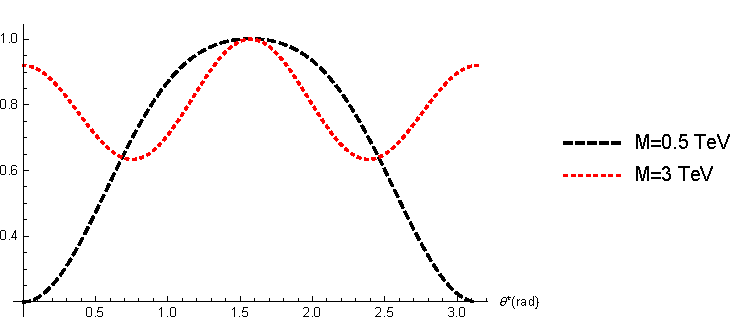
\includegraphics[width=\linewidth]{figures/monojet/comparison_G_mDM10.pdf}
%   \caption{Angular distributions of the total production for 0.5~\tev and 3~\tev graviton mediators for $\mDM=10$~\gev.}
% \end{figure}

% Below a few~\tev in mediator mass, production of a graviton with universal couplings is dominantly gluon-initiated. For heavy mediators, however, up to half of the production occurs through a qq-initiated diagram, leading to a large forward-peaked component of the production \cite{Allanach:2002gn}. For example, Fig.~\ref{fig:gravitoncomparison} shows a calculation of the angular distributions of the total production for 0.5~\tev and 3~\tev graviton mediators in the light WIMP limit ($\mDM=10$~\gev). 